\chapter{Experiments and Results}
This chapter reports the results of the experiments on imbalanced medical/healthcare datasets in detail. Section 4.1 introduces the datasets used as input. This is followed by section 4.2, which reports the results of all the experiments. Section 4.2.1 presents an overall comparison of all class imbalance classification models. Section 4.2.2 and section 4.2.3 illustrates the result of whether a different imbalanced ratio and the different size of the data set have an impact on the performance of the model. Moreover, in section 4.3, the effectiveness of all components in the DDAE is described. 

\section{Input-Data Used}
\subsection{Source of Datasets}
Eight datasets were collected from the medical or healthcare sector. These are Yeast1vs7, Euthyroid Sick, Thyroid Sick, and Mammographic (MGC), Wisconsin Diagnosis Breast Cancer(WDBC) and Pima Indian Diabetes(PID) from UCI \cite{97}, and two sub datasets of Protein Homology (PH1 and PH2) from KDD Cup 2004 \cite{109}, which are utilized to test the performance of these models. The detail of these datasets is depicted in Table \ref{tab6}. In addition, eight further datasets are employed, including Cm1, Mw1, Pc1, Pc3, Pc4 which are from NASA Metrics Data Program (NASA) dataset \cite{110}, Poker89vs6 and Poker8vs6, which are from KEEL \cite{98}, and Optical Recognition of Handwritten Digits (optdigits) from UCI. All these datasets are imbalanced distributed but with various imbalance ratio(IR), instances and features. The detail of these datasets is depicted in Table \ref{tab25}.

Euthyroid Sick and Thyroid Sick record the patient information of the thyroid disease. In Mammographic (MGC), according to the attributes of BI-RADS and the age of patients, breast and benign breast masses are distinguished. Wisconsin Diagnosis Breast Cancer(WDBC) records the data about diagnostic Wisconsin breast cancer. Pima Indian Diabetes(PID) records the patient information of diabetes disease, and all patients here are females at least 21 years old of Pima Indian heritage. Protein Homology dataset consists of the recording about protein homology. Yeast1vs7 contains the data about  the cellular localization sites of proteins. Poker8v6 and Poker89vs6 are used for poker hands prediction. In addition, optdigits contains normalized bitmaps of handwritten digits from a preprinted form.

\begin{table}[h]
    \centering
    \begin{tabular}{|p{0.2\textwidth}<{\centering}|p{0.15\textwidth}<{\centering}|p{0.2\textwidth}<{\centering}|p{0.1\textwidth}<{\centering}|p{0.15\textwidth}<{\centering}|}
    \hline
    \textbf{Dataset}        & \textbf{\#Class} & \textbf{\#Instances} & \textbf{\#F} & \textbf{IR} \\ \hline
    \textbf{Euthyroid Sick} & 2                & 3,163                & 42           & 9.795       \\ \hline
    \textbf{Thyroid Sick}   & 2                & 3,772                & 52           & 15.329      \\ \hline
    \textbf{PH1}            & 2                & 11,274               & 74           & 7.699       \\ \hline
    \textbf{PH2}            & 2                & 31,296               & 74           & 23.148      \\ \hline
    \textbf{MGC}            & 2                & 11,183               & 6            & 42.012      \\ \hline
    \textbf{Yeast1vs7}      & 2                & 459                  & 7            & 14.3        \\ \hline
    \textbf{WDBC}      & 2                & 768                  & 8            & 1.866        \\ \hline
    \textbf{PID}      & 2                & 568                  & 32            & 1.684        \\ \hline
    \end{tabular}
    \caption{Characteristics of used Datasets from Medical or Healthcare Sector}
    \label{tab6}
\end{table}

\begin{table}[h]
    \centering
    \begin{tabular}{|p{0.2\textwidth}<{\centering}|p{0.15\textwidth}<{\centering}|p{0.2\textwidth}<{\centering}|p{0.1\textwidth}<{\centering}|p{0.15\textwidth}<{\centering}|}
    \hline
    \textbf{Dataset}        & \textbf{\#Class} & \textbf{\#Instances} & \textbf{\#F} & \textbf{IR} \\ \hline
    \textbf{optdigits}           & 2                & 5,620                & 65           & 9.144       \\ \hline
    \textbf{Cm1}            & 2                & 497                  & 21           & 9.354       \\ \hline
    \textbf{Mw1}            & 2                & 403                  & 37           & 12          \\ \hline
    \textbf{Pc1}            & 2                & 1109                 & 21           & 13.4        \\ \hline
    \textbf{Pc3}            & 2                & 1563                 & 37           & 8.769       \\ \hline
    \textbf{Pc4}            & 2                & 1458                 & 37           & 7.191       \\ \hline
    \textbf{Poker89vs6}     & 2                & 1485                 & 10           & 58.4        \\ \hline
    \textbf{Poker8vs6}      & 2                & 1477                 & 10           & 85.882      \\ \hline
    \end{tabular}
    \caption{Characteristics of used Datasets from Other Fields}
    \label{tab25}
\end{table}

\subsection{Data Pre-processing}
As described in section 2.1, the datasets in the real world are generally not as perfect as expected. They can be unreliable or dirty, with lack of attribute values, containing noise (errors or outliers) and inconsistent or duplicate values \cite{82}. The performance of classifiers is dependent on the quality of training data. A dirty or incorrect training set can result in a poor classification model \cite{81}. In order to reduce the impact of these issues on prediction models, data pre-processing, a critical part of data analysis and machine learning, takes a huge amount of time \cite{77}. In this paper, the experiment focuses on the performance of the model, so here only a brief pre-processing is performed on the input datasets.

In \cite{77}, the process of data preparation is depicted in four steps: data integration, data cleaning, data normalization and data transformation. However in other literature, such as \cite{79}, this process is presented more detail and data normalization is seen as a part of data transformation. 

When the data is obtained from multiple data sources, step one is critical wherein all the data collected needs to be integrated \cite{77}. This procedure involves the identification of redundant attributes, in which the size of dataset can be decreased, also reducing the modeling time of further algorithms \cite{77}, as well as the detection of duplication and inconsistency. As some identical instances are seen as different due to errors in the entry step, duplication is a cause of inconsistency which means detection is indispensable \cite{80}.

Data cleaning is performed to deal with dirty data \cite{77}, which includes missing values, incorrect data and data with non-standard representation. A high proportion of this kind of data lead to an ineffective and unreliable algorithm \cite{81}. This procedure can be divided into three parts: missing value processing, outliers processing and noise processing \cite{79}.
\begin{figure}[h]
    \centering 
    \begin{minipage}{0.45\textwidth}
        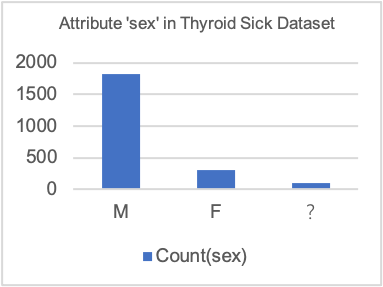
\includegraphics[width=\textwidth]{images/fig9}
        \caption{Distribution of Attribute `sex' in Thyroid Sick Dataset}
        \label{fig9}
    \end{minipage}
    \quad
    \begin{minipage}{0.45\textwidth}
        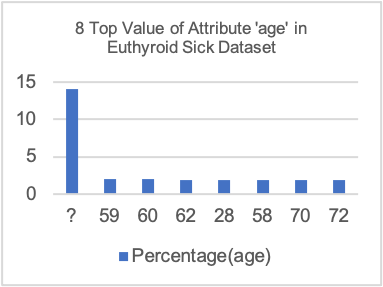
\includegraphics[width=\textwidth]{images/fig10}
        \caption{8 Top Values of Attribute `age' in Euthyroid Sick Dataset}
        \label{fig10}
    \end{minipage}
\end{figure}

In the real world, during the process of acquiring information and data, there will be various causes of data loss and vacancies. There are several options for filling in the missing value. If the missing rate of an attribute is high, this attribute can be deleted directly, so-called listwise deletion \cite{84}. Alternatively, the missing values can be set to specific values calculated on the training set, such as zero, the mean, the median, etc. \cite{85}. For instance, in the Euthyroid Sick Dataset, the missing rate of the attribute `Age' is 14.10\% (466 of 3163). Figure \ref{fig10} shows the 8 top values of this attribute, with the age range of the whole dataset between 1 and 98 years old. During the data cleaning process, this kind of missing value will be replaced with the median of this attribute. Dummy variable adjustment \cite{83} is utilized when the attribute is discrete and has few different values, which can be converted into a dummy variable. For example, in the Thyroid Sick dataset, there are three different values for the gender SEX attribute: `M\footnotemark[11]', `F\footnotemark[12]', `?\footnotemark[13]' (see Figure \ref{fig9}, so this column can be converted into IS\_SEX\_MALE, IS\_SEX\_FEMALE, IS\_SEX\_NA.
\begin{figure}[h]
    \centering 
    \begin{minipage}{0.45\textwidth}
        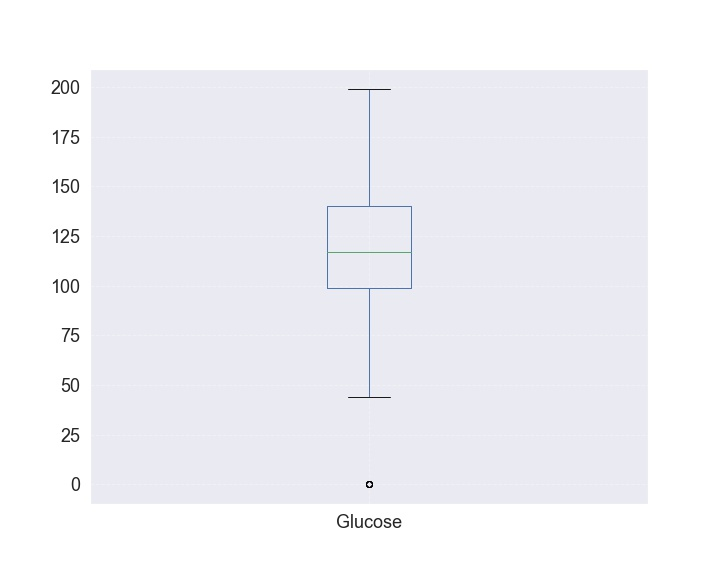
\includegraphics[width=\textwidth]{images/fig11}
        \caption{Box Plot for Attribute `Glucose' in PID Dataset}
        \label{fig11}
    \end{minipage}
    \quad
    \begin{minipage}{0.45\textwidth}
        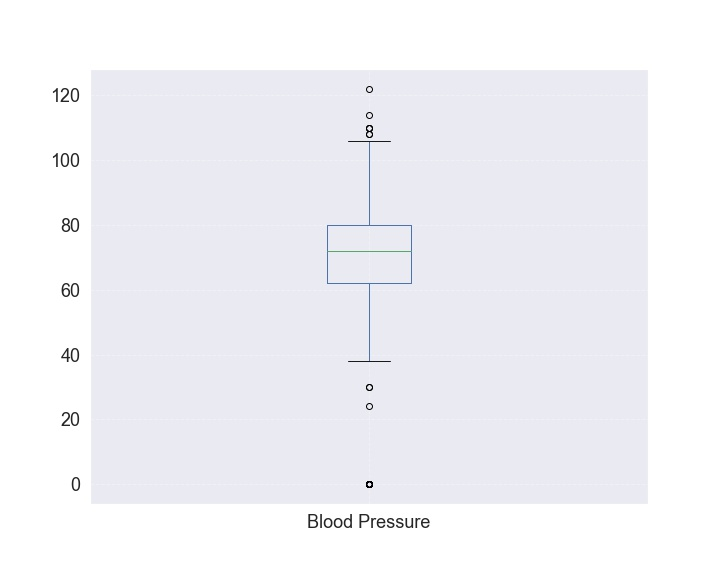
\includegraphics[width=\textwidth]{images/fig12}
        \caption{Box Plot for Attribute `Blood Pressure' in PID Dataset}
        \label{fig12}
    \end{minipage}
\end{figure}

\footnotetext[11]{Male}
\footnotetext[12]{Female}
\footnotetext[13]{Missing Value}

Another kind of data that needs to be cleaned is outlier. Outliers are data points that differ from the rest of the data due to human error, mechanical faults, instrument errors etc. \cite{89}, which is viewed as a normal state of data distribution, and this kind of data outside a specific distribution area or range is also defined as anomalies or abnormalities \cite{88}. One of the visualization methods applied to detect this is box plot using quantiles. Figure \ref{fig11} and Figure \ref{fig12} depict the box plots for the attributes `Blood Pressure' and `Glucose' from the PID dataset. The outliers can be observed clearly in this illustration. There are some instances with an extremely low value for `Blood Pressure' which is rare in the real world. An instance of a 0 `Glucose' can also be viewed as an outlier. Such incorrect data, or data that violates common sense, may lead to an ineffective model. 


There may be variation in the scales of different data features and in the differences between the values \cite{85}. Note the case in the WDBC dataset: the attribute `area\_mean' ranges from 143.5 to 2,501 but the attribute `smoothness\_mean' only ranges from 0.053 to 0.163. This phenomenon may have an impact on the results of data analysis, especially the distance-based algorithms, such as SVM. The data must also be measured to a certain ratio such that they fall into a particular field for detailed analysis \cite{77}. Three normalization procedures \cite{77,78,85} utilized for an attribute $a$ generally are:

Min-Max Normalization\footnotemark[14]\hspace{50pt}$v^{\prime}=\dfrac{v-\min _{a}}{\max _{a}-\min _{a}}\left(n e w_{\max _{a}}-n e w_{\min _{a}}\right)+n e w_{\min _{a}}$
\footnotetext[14]{All the numerical values of the specific numerical attribute $a$ are scaled to a specific range $\left[n e w_{\min _{a}}, n e w_{\max _{a}}\right]$}

Z-score Normalization\footnotemark[15]\hspace{150pt}$v^{\prime}=\dfrac{v-m e a n_{a}}{s t a n d_{-} d e v_{a}}$
\footnotetext[15]{$mean_{a}$ is the sample mean and ${stand\_dev}_{a}$ is the sample standard deviation, which is computed as $\dfrac{1}{n} \sum_{i=1}^{n}\left|v_{i}-mean_{a}\right|$}

Decimal Scaling Normalization\footnotemark[16]\hspace{130pt}$v^{\prime}=\dfrac{v}{10^{j}}$
\footnotetext[16]{where $j$ is the smallest integer such that $n e w_{\max _{a}}<1$}

\begin{table}[h]
    \centering
    \begin{tabular}{|c|c|c|c|c|c|c|}
    \cline{1-2} \cline{4-7}
    \textbf{Raw Number} & \textbf{referral source} & \multirow{6}{*}{$\Longrightarrow$} & \textbf{RSource1} & \textbf{RSource2} & \textbf{RSource3} & \textbf{RSource4} \\ \cline{1-2} \cline{4-7} 
    1                   & SVI                      &                        & 1                 & 0                 & 0                 & 0                 \\ \cline{1-2} \cline{4-7} 
    2                   & STMW                     &                        & 0                 & 0                 & 1                 & 0                 \\ \cline{1-2} \cline{4-7} 
    3                   & SVHD                     &                        & 0                 & 0                 & 0                 & 1                 \\ \cline{1-2} \cline{4-7} 
    4                   & SVHC                     &                        & 0                 & 1                 & 0                 & 0                 \\ \cline{1-2} \cline{4-7} 
    5                   & other                    &                        & 0                 & 0                 & 0                 & 0                 \\ \cline{1-2} \cline{4-7} 
    \end{tabular}
    \caption{Comparison of Before and After One Hot Encoding for Attribute `referral source' in Thyroid Sick Dataset}
    \label{tab7}
\end{table}

Other useful steps are feature encoding \cite{85}, feature selection \cite{87}, dimensionality reduction \cite{85} etc. Since most models have a preference for processing numerical data, handling some text and categorical attributes, feature encoding is a kind of useful data transformation to make data more acceptable as input for models \cite{85}. The attribute `referral source' of thyroid sick dataset contains five values: `SVI', `SVHC', `STMW', `SVHD' and `other'. Table \ref{tab7} shows an example of this attribute before and after transformation. This attribute will be replaced by four new attributes: `RSource1', `RSource2', `RSource3' and `RSource4'. This is also an application of dummy variables adjustment and those new attributes are called dummy attributes. The package Scikit-Learn provides a OneHotEncoder class to transform these kinds of category values into one-hot vectors \cite{85}.

There is no set series of specific data pre-processing methods that can be applied to all data sets, so for different datasets, specific analysis needs to be carried out according to its characteristics \cite{80}.

\subsection{Split of Dataset into Training Set and Testing Set}
For evaluating machine learning algorithms, the Train-Test Split is indispensable, which involves the division of a given dataset into two subset according to a specific ratio. The subset applied to fit the algorithm is called the training set, and the other is referred to as the testing set and is utilized to evaluate the fit algorithm \cite{102}. To be exact, available data with known input vector and target values works on fitting the given model, so that it can predict new instances without class values. In this paper, all the given datasets will be split based on Train:Test = 7:3.

\section{Results on All Models}
\subsection{Overall Comparison}
Tables \ref{tab8}-\ref{tab17} are provided for each separate dataset, listing the performance of each of the models applied in terms of G-mean, F1 and AUCPRC. 

\begin{table}[h]
    \centering
    \begin{tabular}{|p{0.2\textwidth}<{\centering}|p{0.2\textwidth}<{\centering}|p{0.2\textwidth}<{\centering}|p{0.2\textwidth}<{\centering}|}
    \hline
    \multirow{2}{*}{Models} & \multicolumn{3}{c|}{\textbf{Euthyroid Sick}}    \\ \cline{2-4} 
                             & \textbf{G-mean} & \textbf{F1} & \textbf{AUCPRC} \\ \hline
    DDAE                     & 0.880	&0.552	&0.587                \\ \hline
    MWMOTE                   & 0.832	&0.658	&0.616                 \\ \hline
    SMOTE                    & 0.829	&0.667	&0.621                 \\ \hline
    RUSBoost                 & 0.911	&0.725	&0.779                 \\ \hline
    AdaBoost                 & 0.904	&\textbf{0.862}	&\textbf{0.901}                 \\ \hline
    MetaCost                 & 0.935	&0.846	&0.723               \\ \hline
    csDCT                    & 0.960	&0.846	&0.723                 \\ \hline
    CAdaMEC                  & 0.876	&0.831	&0.865                 \\ \hline
    self-paced               & \textbf{0.971}	&0.856	&0.861                 \\ \hline
    IML                      & 0.867	&0.809	&0.836                \\ \hline\hline
    \textbf{Average}         & 0.897	&0.765	&0.751                 \\ \hline
    \end{tabular}
    \caption{Overall Results for Euthyroid Sick Dataset}
    \label{tab8}
\end{table}
%%%%%
\begin{table}[h]
    \centering
    \begin{tabular}{|p{0.2\textwidth}<{\centering}|p{0.2\textwidth}<{\centering}|p{0.2\textwidth}<{\centering}|p{0.2\textwidth}<{\centering}|}
    \hline
    \multirow{2}{*}{Models} & \multicolumn{3}{c|}{\textbf{Thyroid Sick}}    \\ \cline{2-4} 
                             & \textbf{G-mean} & \textbf{F1} & \textbf{AUCPRC} \\ \hline
    DDAE                     & 0.883	&0.506	&0.622               \\ \hline
    MWMOTE                   &0.735	&0.558	&0.342                \\ \hline
    SMOTE                    & 0.694	&0.535	&0.323                \\ \hline
    RUSBoost                 & 0.908	&0.783	&0.805                \\ \hline
    AdaBoost                 & 0.879	&0.828	&0.882                \\ \hline
    MetaCost                 & 0.413	&0.280	&0.342               \\ \hline
    csDCT                    & 0.891	&0.811	&0.700                \\ \hline
    CAdaMEC                  & 0.835	&0.794	&\textbf{0.901}                \\ \hline
    self-paced               & \textbf{0.915}	&\textbf{0.861}	&0.893                 \\ \hline
    IML                      & 0.615	&0.474	&0.335               \\ \hline\hline
    \textbf{Average}         & 0.777	&0.643	&0.615                 \\ \hline
    \end{tabular}
    \caption{Overall Results for Thyroid Sick Dataset}
    \label{tab9}
\end{table}
%%%%
\begin{table}[H]
    \centering
    \renewcommand\arraystretch{0.85}
    \begin{tabular}{|p{0.2\textwidth}<{\centering}|p{0.2\textwidth}<{\centering}|p{0.2\textwidth}<{\centering}|p{0.2\textwidth}<{\centering}|}
    \hline
    \multirow{2}{*}{Models} & \multicolumn{3}{c|}{\textbf{PH1}}    \\ \cline{2-4} 
                             & \textbf{G-mean} & \textbf{F1} & \textbf{AUCPRC} \\ \hline
    DDAE                     & \textbf{0.955}	&0.828	&0.891               \\ \hline
    MWMOTE                   &0.934	&0.781	&0.647                \\ \hline
    SMOTE                    & 0.925	&0.765	&0.630                \\ \hline
    RUSBoost                 & 0.938	&0.868	&0.940                \\ \hline
    AdaBoost                 & 0.940	&\textbf{0.926}	&\textbf{0.963}                \\ \hline
    MetaCost                 & 0.851	&0.774	&0.706               \\ \hline
    csDCT                    & 0.918	&0.837	&0.728                \\ \hline
    CAdaMEC                  & 0.934	&0.913	&0.960               \\ \hline
    self-paced               & 0.936	&0.892	&0.943                 \\ \hline
    IML                      & 0.907	&0.874	&0.925               \\ \hline\hline
    \textbf{Average}         & 0.924	&0.846	&0.833                 \\ \hline
    \end{tabular}
    \vspace{-8pt}
    \caption{Overall Results for PH1 Dataset}
    \label{tab10}
\end{table}
%%%%%
\begin{table}[h]
    \centering
    \begin{tabular}{|p{0.2\textwidth}<{\centering}|p{0.2\textwidth}<{\centering}|p{0.2\textwidth}<{\centering}|p{0.2\textwidth}<{\centering}|}
    \hline
    \multirow{2}{*}{Models} & \multicolumn{3}{c|}{\textbf{PH2}}    \\ \cline{2-4} 
                             & \textbf{G-mean} & \textbf{F1} & \textbf{AUCPRC} \\ \hline
    DDAE                     & 0.986	&0.830	&0.956               \\ \hline
    MWMOTE                   &0.953	&0.664	&0.498               \\ \hline
    SMOTE                    & 0.935	&0.701	&0.546               \\ \hline
    RUSBoost                 &0.996	&0.981	&0.999              \\ \hline
    AdaBoost                 & 0.995	&0.994	&\textbf{1}                \\ \hline
    MetaCost                 & 0.884	&0.794	&0.783               \\ \hline
    csDCT                    & \textbf{0.999}	&\textbf{0.999}	&0.997                \\ \hline
    CAdaMEC                  & 0.995	&0.991	&\textbf{1}               \\ \hline
    self-paced               & \textbf{0.999}	&\textbf{0.999}	&\textbf{1}                 \\ \hline
    IML                      & 0.978	&0.964	&0.999              \\ \hline\hline
    \textbf{Average}         & 0.972	&0.892	&0.878                 \\ \hline
    \end{tabular}
    \vspace{-8pt}
    \caption{Overall Results for PH2 Dataset}
    \label{tab11}
\end{table}
%%%%%
\begin{table}[h]
    \centering
    \renewcommand\arraystretch{0.95} 
    \begin{tabular}{|p{0.2\textwidth}<{\centering}|p{0.2\textwidth}<{\centering}|p{0.2\textwidth}<{\centering}|p{0.2\textwidth}<{\centering}|}
    \hline
    \multirow{2}{*}{Models} & \multicolumn{3}{c|}{\textbf{optdigits}}    \\ \cline{2-4} 
                             & \textbf{G-mean} & \textbf{F1} & \textbf{AUCPRC} \\ \hline
    DDAE                     & \textbf{0.986}	&0.904	&\textbf{0.995}               \\ \hline
    MWMOTE                   &\textbf{0.986}	&0.965	&0.934              \\ \hline
    SMOTE                    & 0.983	&0.968	&0.940               \\ \hline
    RUSBoost                 &0.970	&0.921	&0.971              \\ \hline
    AdaBoost                 & 0.963	&0.955	&0.986               \\ \hline
    MetaCost                 & 0.836	&0.616	&0.490               \\ \hline
    csDCT                    & 0.900	&0.758	&0.637                \\ \hline
    CAdaMEC                  & 0.972	&\textbf{0.985}	&0.992               \\ \hline
    self-paced               & 0.965	&0.946	&0.980                \\ \hline
    IML                      & 0.981	&0.970	&\textbf{0.995}             \\ \hline\hline
    \textbf{Average}         & 0.954	&0.899	&0.892                \\ \hline
    \end{tabular}
    \vspace{-8pt}
    \caption{Overall Results for optdigits Dataset}
    \label{tab12}
\end{table}
%%%%%
\begin{table}[H]
    \centering
    \renewcommand\arraystretch{0.85}
    \begin{tabular}{|p{0.2\textwidth}<{\centering}|p{0.2\textwidth}<{\centering}|p{0.2\textwidth}<{\centering}|p{0.2\textwidth}<{\centering}|}
    \hline
    \multirow{2}{*}{Models} & \multicolumn{3}{c|}{\textbf{MGC}}    \\ \cline{2-4} 
                             & \textbf{G-mean} & \textbf{F1} & \textbf{AUCPRC} \\ \hline
    DDAE                     & \textbf{0.878}	&0.321	&0.324               \\ \hline
    MWMOTE                   &0.798	&0.522	&0.321              \\ \hline
    SMOTE                    & 0.813	&0.539	&0.331               \\ \hline
    RUSBoost                 &0.708	&0.549	&0.513              \\ \hline
    AdaBoost                 & 0.803	&\textbf{0.767}	&\textbf{0.758}               \\ \hline
    MetaCost                 & 0.793	&0.313	&0.208               \\ \hline
    csDCT                    & 0.782	&0.284	&0.141               \\ \hline
    CAdaMEC                  & 0.640	&0.562	&0.627               \\ \hline
    self-paced               & 0.877	&0.516	&0.669                \\ \hline
    IML                      & 0.411	&0.286	&0.270             \\ \hline\hline
    \textbf{Average}         & 0.750	&0.466	&0.416                \\ \hline
    \end{tabular}
    \vspace{-8pt}
    \caption{Overall Results for MGC Dataset}
    \label{tab13}
\end{table}
\vspace{-13pt}
%%%%%
\begin{table}[h]
    \centering
    \begin{tabular}{|p{0.2\textwidth}<{\centering}|p{0.2\textwidth}<{\centering}|p{0.2\textwidth}<{\centering}|p{0.2\textwidth}<{\centering}|}
    \hline
    \multirow{2}{*}{Models} & \multicolumn{3}{c|}{\textbf{WDBC}}    \\ \cline{2-4} 
                             & \textbf{G-mean} & \textbf{F1} & \textbf{AUCPRC} \\ \hline
    DDAE                     & 0.866	&0.831	&0.825               \\ \hline
    MWMOTE                   &0.891	&0.873	&\textbf{0.957}              \\ \hline
    SMOTE                    & \textbf{0.941}	&\textbf{0.937}	&0.945               \\ \hline
    RUSBoost                 &0.911	&0.898	&0.926              \\ \hline
    AdaBoost                 & 0.887	&0.871	&0.832               \\ \hline
    MetaCost                 & 0.887	&0.871	&0.910              \\ \hline
    csDCT                    & 0.907	&0.882	&0.831               \\ \hline
    CAdaMEC                  & 0.891	&0.873	&\textbf{0.957}               \\ \hline
    self-paced               & 0.866	&0.831	&0.825                \\ \hline
    IML                      & 0.893	&0.870	&0.910             \\ \hline\hline
    \textbf{Average}         & 0.894	&0.874	&0.892               \\ \hline
    \end{tabular}
    \vspace{-8pt}
    \caption{Overall Results for WDBC Dataset}
    \label{tab14}
\end{table}
\vspace{-13pt}
%%%%%
\begin{table}[h]
    \centering
    \renewcommand\arraystretch{0.95} 
    \begin{tabular}{|p{0.2\textwidth}<{\centering}|p{0.2\textwidth}<{\centering}|p{0.2\textwidth}<{\centering}|p{0.2\textwidth}<{\centering}|}
    \hline
    \multirow{2}{*}{Models} & \multicolumn{3}{c|}{\textbf{PID}}    \\ \cline{2-4} 
                             & \textbf{G-mean} & \textbf{F1} & \textbf{AUCPRC} \\ \hline
    DDAE                     & 0.712	&0.657	&0.586               \\ \hline
    MWMOTE                   &0.760	&0.780	&0.841             \\ \hline
    SMOTE                    & \textbf{0.807}	&\textbf{0.824}	&\textbf{0.859}               \\ \hline
    RUSBoost                 &0.649	&0.562	&0.642             \\ \hline
    AdaBoost                 & 0.693	&0.671	&0.709               \\ \hline
    MetaCost                 & 0.751	&0.688	&0.734             \\ \hline
    csDCT                    &0.738	&0.671	&0.610              \\ \hline
    CAdaMEC                  & 0.727	&0.658	&0.692               \\ \hline
    self-paced               & 0.640	&0.550	&0.610                \\ \hline
    IML                      & 0.667	&0.587	&0.586             \\ \hline\hline
    \textbf{Average}         & 0.714	&0.665	&0.687               \\ \hline
    \end{tabular}
    \vspace{-8pt}
    \caption{Overall Results for PID Dataset}
    \label{tab15}
\end{table}
%%%%%
\begin{table}[H]
    \centering
    \renewcommand\arraystretch{0.85}
    \begin{tabular}{|p{0.2\textwidth}<{\centering}|p{0.2\textwidth}<{\centering}|p{0.2\textwidth}<{\centering}|p{0.2\textwidth}<{\centering}|}
    \hline
    \multirow{2}{*}{Models} & \multicolumn{3}{c|}{\textbf{Yeast1vs7}}    \\ \cline{2-4} 
                             & \textbf{G-mean} & \textbf{F1} & \textbf{AUCPRC} \\ \hline
    DDAE                     & 0.713	&0.214	&0.257               \\ \hline
    MWMOTE                   &\textbf{0.778}	&0.307	&0.336             \\ \hline
    SMOTE                    &0.775	&0.300	&\textbf{0.468}               \\ \hline
    RUSBoost                 &0.598	& 0.353	&0.304            \\ \hline
    AdaBoost                 & 0.496	&0.333	&0.305              \\ \hline
    MetaCost                 & 0.331	&0.080	&0.083             \\ \hline
    csDCT                    &0	&0	&0.129              \\ \hline
    CAdaMEC                  &0	&0	&0.066              \\ \hline
    self-paced               & 0.740	&0.245	&0.181               \\ \hline
    IML                      & 0.607	&\textbf{0.526}	&0.387             \\ \hline\hline
    \textbf{Average}         & 0.582	&0.237	&0.304               \\ \hline
    \end{tabular}
    \vspace{-8pt}
    \caption{Overall Results for Yeast1vs7 Dataset}
    \label{tab16}
\end{table}
%%%%%
\begin{table}[h]
    \centering
    \vspace{-13pt}
    \begin{tabular}{|p{0.2\textwidth}<{\centering}|p{0.2\textwidth}<{\centering}|p{0.2\textwidth}<{\centering}|p{0.2\textwidth}<{\centering}|}
    \hline
    \multirow{2}{*}{Models} & \multicolumn{3}{c|}{\textbf{Poker8vs6}}    \\ \cline{2-4} 
                             & \textbf{G-mean} & \textbf{F1} & \textbf{AUCPRC} \\ \hline
    DDAE                     &0.622	&0.029	&0.078              \\ \hline
    MWMOTE                   &0.866	&0.857	&0752            \\ \hline
    SMOTE                    &0.999	&0.889	&0.800               \\ \hline
    RUSBoost                 &0.707	&0.667	&0.761            \\ \hline
    AdaBoost                 & \textbf{1}	&\textbf{1}	&\textbf{1}             \\ \hline
    MetaCost                 & 0	&0	&0             \\ \hline
    csDCT                    &0.443	&0.019	&0.009              \\ \hline
    CAdaMEC                  &  0	&0	&0.007              \\ \hline
    self-paced               & 0.613	&0.085	&0.038              \\ \hline
    IML                      & 0.500	&0.400	&0.379             \\ \hline\hline
    \textbf{Average}         & 0.695	&0.523	&0.482               \\ \hline
    \end{tabular}
    \vspace{-8pt}
    \caption{Overall Results for Poker8vs6 Dataset}
    \label{tab17}
\end{table}
\vspace{-20pt}
%%%%%
\begin{table}[h]
    \centering
    \begin{tabular}{|p{0.2\textwidth}<{\centering}|p{0.2\textwidth}<{\centering}|p{0.2\textwidth}<{\centering}|p{0.2\textwidth}<{\centering}|}
    \hline
    \multirow{2}{*}{Models} & \multicolumn{3}{c|}{\textbf{Poker89vs6}}    \\ \cline{2-4} 
                             & \textbf{G-mean} & \textbf{F1} & \textbf{AUCPRC} \\ \hline
    DDAE                     &0.704	&0.051	&0.188             \\ \hline
    MWMOTE                   &0.986	&0.500	&0.750             \\ \hline
    SMOTE                    &0.979	&0.400	&0.750               \\ \hline
    RUSBoost                 &\textbf{1}	&\textbf{1}	&\textbf{1}             \\ \hline
    AdaBoost                 & \textbf{1}	&\textbf{1}	&\textbf{1}             \\ \hline
    MetaCost                 & 0	&0	&0.015             \\ \hline
    csDCT                    &0.495	&0.032	&0.019              \\ \hline
    CAdaMEC                  &   0	&0	&0.014           \\ \hline
    self-paced               & 0.567	&0.036	&0.016              \\ \hline
    IML                      & 0.816	&0.800	&0.848            \\ \hline\hline
    \textbf{Average}         & 0.755	&0.482	&0.559               \\ \hline
    \end{tabular}
    \vspace{-8pt}
    \caption{Overall Results for Poker89vs6 Dataset}
    \label{tab18}
\end{table}
%%%%%
\begin{table}[H]
    \centering
    \renewcommand\arraystretch{0.85} 
    \begin{tabular}{|p{0.2\textwidth}<{\centering}|p{0.2\textwidth}<{\centering}|p{0.2\textwidth}<{\centering}|p{0.2\textwidth}<{\centering}|}
    \hline
    \multirow{2}{*}{Models} & \multicolumn{3}{c|}{\textbf{Cm1}}    \\ \cline{2-4} 
                             & \textbf{G-mean} & \textbf{F1} & \textbf{AUCPRC} \\ \hline
    DDAE                     &0.699	&0.29	&0.214             \\ \hline
    MWMOTE                   &0.679	&0.286	&0.182             \\ \hline
    SMOTE                    &0.715	&0.308	&0.219               \\ \hline
    RUSBoost                 &0.438	&0.25	&0.386            \\ \hline
    AdaBoost                 & \textbf{0.981}	&\textbf{0.970}	&\textbf{0.995}             \\ \hline
    MetaCost                 & 0.744	&0.322	&0.198             \\ \hline
    csDCT                    &0.559	&0.203	&0.158              \\ \hline
    CAdaMEC                  &0.622	&0.237	&0.196             \\ \hline
    self-paced               &0.690	&0.298	&0.262              \\ \hline
    IML                      &0.499	&0.207	&0.137            \\ \hline\hline
    \textbf{Average}         &0.663	&0.337	&0.295              \\ \hline
    \end{tabular}
    \vspace{-8pt}
    \caption{Overall Results for Cm1 Dataset}
    \label{tab19}
\end{table}
\vspace{-23.5pt}
%%%%%
\begin{table}[h]
    \centering
    \begin{tabular}{|p{0.2\textwidth}<{\centering}|p{0.2\textwidth}<{\centering}|p{0.2\textwidth}<{\centering}|p{0.2\textwidth}<{\centering}|}
    \hline
    \multirow{2}{*}{Models} & \multicolumn{3}{c|}{\textbf{Pc1}}    \\ \cline{2-4} 
                             & \textbf{G-mean} & \textbf{F1} & \textbf{AUCPRC} \\ \hline
    DDAE                     &\textbf{0.740}	&0.237	&0.179            \\ \hline
    MWMOTE                   &0.718	&0.226	&0.160            \\ \hline
    SMOTE                    &0.734	&0.244	&0.205               \\ \hline
    RUSBoost                 &0.440	&0.235	&0.214            \\ \hline
    AdaBoost                 & 0.223	&0.091	&0.226            \\ \hline
    MetaCost                 & 0.548	&0.197	&0.109            \\ \hline
    csDCT                    &0.642	&0.185	&0.099              \\ \hline
    CAdaMEC                  &0.673	&0.203	&0.156             \\ \hline
    self-paced               &0.649	&\textbf{0.253}	&\textbf{0.251}              \\ \hline
    IML                      &0.649	&\textbf{0.253}	&\textbf{0.251}          \\ \hline\hline
    \textbf{Average}         &0.602	&\textbf{0.212}	&0.185              \\ \hline
    \end{tabular}
    \vspace{-8pt}
    \caption{Overall Results for Pc1 Dataset}
    \label{tab20}
\end{table}
\vspace{-13pt}
%%%%%
\begin{table}[h]
    \centering
    \begin{tabular}{|p{0.2\textwidth}<{\centering}|p{0.2\textwidth}<{\centering}|p{0.2\textwidth}<{\centering}|p{0.2\textwidth}<{\centering}|}
    \hline
    \multirow{2}{*}{Models} & \multicolumn{3}{c|}{\textbf{Pc4}}    \\ \cline{2-4} 
                             & \textbf{G-mean} & \textbf{F1} & \textbf{AUCPRC} \\ \hline
    DDAE                     &0.756	&0.381	&0.364            \\ \hline
    MWMOTE                   &0.825	&0.497	&0.499            \\ \hline
    SMOTE                    &0.789	&0.460	&0.443               \\ \hline
    RUSBoost                 &0.752	&0.418	&0.413           \\ \hline
    AdaBoost                 &0.823	&\textbf{0.699}	&\textbf{0.714}           \\ \hline
    MetaCost                 &0.790	&0.436	&0.273            \\ \hline
    csDCT                    &0.826	&0.512	&0.364             \\ \hline
    CAdaMEC                  &0.831	&0.475	&0.695             \\ \hline
    self-paced               &\textbf{0.837}	&0.524	&0.453            \\ \hline
    IML                      &0.668	&0.505	&0.416          \\ \hline\hline
    \textbf{Average}         &0.790	&0.491	&0.463             \\ \hline
    \end{tabular}
    \vspace{-8pt}
    \caption{Overall Results for Pc4 Dataset}
    \label{tab22}
\end{table}
%%%%%
\begin{table}[H]
    \centering
    \renewcommand\arraystretch{0.85} 
    \begin{tabular}{|p{0.2\textwidth}<{\centering}|p{0.2\textwidth}<{\centering}|p{0.2\textwidth}<{\centering}|p{0.2\textwidth}<{\centering}|}
    \hline
    \multirow{2}{*}{Models} & \multicolumn{3}{c|}{\textbf{Pc3}}    \\ \cline{2-4} 
                             & \textbf{G-mean} & \textbf{F1} & \textbf{AUCPRC} \\ \hline
    DDAE                     &0.772	&0.440	&0.319            \\ \hline
    MWMOTE                   &\textbf{0.780}&\textbf{0.491}&\textbf{0.401} \\ \hline
    SMOTE                    &0.752	&0.440	&0.376               \\ \hline
    RUSBoost                 &0.452	&0.273	&0.310            \\ \hline
    AdaBoost                 &0.438	&0.289	&0.343            \\ \hline
    MetaCost                 &0.737	&0.432	&0.263            \\ \hline
    csDCT                    &0.719	&0.432	&0.284              \\ \hline
    CAdaMEC                  &0.629	&0.301	&0.336             \\ \hline
    self-paced               &0.719	&0.432	&0.284             \\ \hline
    IML                      &0.418	&0.267	&0.300          \\ \hline\hline
    \textbf{Average}         &0.645	&0.380	&0.322             \\ \hline
    \end{tabular}
    \caption{Overall Results for Pc3 Dataset}
    \label{tab21}
\end{table}
%%%%%

What can be observed from these results is that the G-mean of DDAE is close to or better than the average on most of the datasets. For example, the G-mean value obtained on the MGC is 0.878, while the average value at this time is only 0.750; the G-mean value yielded on Pc1 is 0.740, while the figure for RUSBoost is only 0.44. However, it should be noted that DDAE's F1 and AUCPRC are not satisfactory; they are, lower than the corresponding average values on most of the datasets. In comparison, the two ensemble algorithms, AdaBoost and self-paced Ensemble Classifier, can maintain satisfactory F1, AUCPRC under most circumstances, as well as G-mean,showing that these two algorithms can accurately classify not only a large proportion of minority but also most majority in most cases. For example, AdaBoost has achieved the highest F1 and AUCPRC on datasets such as Euthyroid Sick and PH1, its F1 (0.970) being nearly three times that of MetaCost (0.322), which is the second highest value, on the Cm1 dataset; self-paced Ensemble Classifier has achieved the highest F1 and AUCPRC on Thyroid Sick dataset and PH2 dataset, and its F1 and AUCPRC on Pc1 are twice that of AdaBoost. In addition, the performance of another ensemble algorithm, RUSBoost, is relatively stable, with performance on most datasets being close to the average. 

The stability of cost-sensitive learning models, such as MetaCost, csDCT and CAdaMEC, is not very obvious. CAdaMEC, as well as csDCt, performed well on the optdigits dataset and the Thyroid Sick dataset, but on Yeast1vs7 dataset, its performance is the worst. 

SMOTE and MWMOTE are two sampling models, with a similar performance in most cases except on the Poker8vs6 dataset.

Moreover, the performance of IML fluctuates above and below the average level.Compared with other algorithms, the advantage is not obvious.


%%%%%
\begin{table}[h]
    %\centering
    \begin{tabular}{|p{0.1\textwidth}<{\centering}|p{0.06\textwidth}<{\centering}|p{0.06\textwidth}<{\centering}|p{0.06\textwidth}<{\centering}|p{0.06\textwidth}<{\centering}|p{0.06\textwidth}<{\centering}|p{0.06\textwidth}<{\centering}|p{0.06\textwidth}<{\centering}|p{0.06\textwidth}<{\centering}|p{0.06\textwidth}<{\centering}|p{0.06\textwidth}<{\centering}|}
    \hline
    \multirow{2}{*}{Dataset} & \multicolumn{10}{c|}{\textbf{Recall}}    \\ \cline{2-11} 
                             & \tiny\textbf{DDAE} & \tiny\textbf{MWMOTE} & \tiny\textbf{SMOTE} & \tiny\textbf{RUSBoost} & \tiny\textbf{AdaBoost} & \tiny\textbf{MetaCost} & \tiny\textbf{csDCT} & \tiny\textbf{CAdaMEC} &
                            \tiny\textbf{self-paced} & \tiny\textbf{IML}\\ \hline
    Euthyroid Sick                     &\textbf{0.929}&0.737&0.725&0.888&0.827&0.898&0.867&0.776&0.847&0.763\\ \hline
    Thyroid Sick                   
    &\textbf{0.883}&0.558&0.494&0.844&0.779&0.169&0.805&0.701&0.844&0.383\\ \hline
    PH1                    
    &\textbf{0.956}&0.926&0.913&0.900&0.887&0.741&0.867&0.877&0.887&0.831\\ \hline
    PH2                 
    &0.990&0.946&0.939&0.992&0.990&0.787&\textbf{1}&0.990&0.997&0.931\\ \hline
    % optdigits                 
    % &\textbf{0.994}&0.977&0.971&0.953&0.929&0.759&0.847&0.947&0.935&0.965\\ \hline
    MGC                 
    &\textbf{0.834}&0.651&0.675&0.506&0.675&0.675&0.663&0.410&0.795&0.169\\ \hline
    WDBC                    
    &0.894&0.950&\textbf{0.960}&0.864&0.894&0.818&0.909&0.833&0.864&0.864\\ \hline
    PID                  
    &0.810&0.824&\textbf{0.869}&0.512&0.548&0.774&0.690&0.631&0.524&0.524\\ \hline
    Yeast1vs7               
    &\textbf{0.750}&\textbf{0.750}&\textbf{0.750}&0.375&0.250&0.125&0&\textbf{0.750}&\textbf{0.750}&0.375\\ \hline
    \end{tabular}
    \caption{Recall for for All Models on the Nine Medical Public Datasets}
    \label{tab23}
\end{table}
In order to investigate the ability of theses models mentioned in this paper on positive sample detection, which is important for the field of medical or healthcare, the recall for all these models are presented in Table \ref{tab23}.  

It can be observed that the recall for DDAE performs well on all medical datasets. The recall for self-paced Ensemble Classifier and CAdaMEC can also maintain a relatively stable performance on nearly all the medical datasets.
\begin{table}[h]
    %\centering
    \footnotesize
    \begin{tabular}{|p{0.1\textwidth}<{\centering}|p{0.06\textwidth}<{\centering}|p{0.06\textwidth}<{\centering}|p{0.06\textwidth}<{\centering}|p{0.06\textwidth}<{\centering}|p{0.06\textwidth}<{\centering}|p{0.06\textwidth}<{\centering}|p{0.06\textwidth}<{\centering}|p{0.06\textwidth}<{\centering}|p{0.06\textwidth}<{\centering}|p{0.06\textwidth}<{\centering}|}
    \hline
    \multirow{2}{*}{Dataset} & \multicolumn{10}{c|}{\textbf{Learning Time (in Seconds)}}    \\ \cline{2-11} 
                             & \tiny\textbf{DDAE} & \tiny\textbf{MWMOTE} & \tiny\textbf{SMOTE} & \tiny\textbf{RUSBoost} & \tiny\textbf{AdaBoost} & \tiny\textbf{MetaCost} & \tiny\textbf{csDCT} & \tiny\textbf{CAdaMEC} &
                            \tiny\textbf{self-paced} & \tiny\textbf{IML}\\ \hline
                          
    Euthyroid Sick                     &146.775&0.381&0.224&0.050&0.110&2.426&7.586&0.185&\textbf{0.041}&912.874\\ \hline
    Thyroid Sick                   
    &471.882&1.362&1.711&0.542&1.103&19.91&16.786&0.370&\textbf{0.08}&1680.46\\ \hline
    PH1                    
    &1753.42&0.940&8.006&4.857&2.494&64.927&786.164&1.053&\textbf{0.226}&16627.12\\ \hline
    PH2                 
    &14446.34&115.313&51.917&4.091&5.783&188.748&4513.89&2.770&\textbf{0.302}&46155.96\\ \hline
    optdigits                 
    &637.385&0.983&3.207&0.863&0.976&31.625&166.284&0.372&\textbf{0.07}&5001.329\\ \hline
    MGC                 
    &1472.36&0.845&0.749&0.529&0.679&54.577&31.973&0.231&\textbf{0.065}&9861.933\\ \hline
    WDBC                    
    &13.426&0.950&0.960&\textbf{0.864}&0.894&0.818&0.909&16.117&\textbf{0.864}&8.106\\ \hline
    PID                  
    &17.45&0.381&0.224&0.381&0.478&9.187&15.547&0.089&\textbf{0.029}&27.034\\ \hline
    Yeast1vs7               
    &46.994&0.083&\textbf{0.014}&0.235&0.141&2.411&11.044&0.109&0.036&5.85\\ \hline
    Cm1               
    &54.638&0.069&0.060&\textbf{0.016}&0.106&1.201&36.415&0.086&0.029&10.873\\ \hline
    Pc1               
    &76.463&0.103&0.119&0.244&0.177&3.57&35.073&0.106&\textbf{0.032}&8.702\\ \hline
    Pc3              
    &110.98&0.358&0.053&0.274&0.258&5.388&136.251&0.157&\textbf{0.034}&180.428\\ \hline
    Pc4               
    &97.79&0.399&0.638&0.259&0.208&5.175&65.156&0.118&\textbf{0.038}&156.004\\ \hline
    Poker8vs6               
    &126.932&0.101&\textbf{0.034}&0.185&0.135&4.565&7.267&0.090&0.038&134.869\\ \hline
    Poker89vs6               
    &101.163&0.136&\textbf{0.020}&0.236&0.261&4.617&6.322&0.102&0.029&135.836\\ \hline
    \end{tabular}
    \caption{Learning Time for All Models on the Public Datasets}
    \label{tab24}
\end{table}

\begin{table}[h]
    %\centering
    \footnotesize
    \begin{tabular}{|p{0.1\textwidth}<{\centering}|p{0.06\textwidth}<{\centering}|p{0.06\textwidth}<{\centering}|p{0.06\textwidth}<{\centering}|p{0.06\textwidth}<{\centering}|p{0.06\textwidth}<{\centering}|p{0.06\textwidth}<{\centering}|p{0.06\textwidth}<{\centering}|p{0.06\textwidth}<{\centering}|p{0.06\textwidth}<{\centering}|p{0.06\textwidth}<{\centering}|}
    \hline
    \multirow{2}{*}{Dataset} & \multicolumn{10}{c|}{\textbf{Memory Usage (in MB)}}    \\ \cline{2-11} 
                             & \tiny\textbf{DDAE} & \tiny\textbf{MWMOTE} & \tiny\textbf{SMOTE} & \tiny\textbf{RUSBoost} & \tiny\textbf{AdaBoost} & \tiny\textbf{MetaCost} & \tiny\textbf{csDCT} & \tiny\textbf{CAdaMEC} &
                            \tiny\textbf{self-paced} & \tiny\textbf{IML}\\ \hline
                          
    Euthyroid Sick                     &1.587&0.833&0.388&0.417&\textbf{0.342}&0.418&1.449&0.369&0.399&0.977\\ \hline
    Thyroid Sick                   
    &1.978&0.425&0.362&0.403&\textbf{0.344}&0.41&0.956&0.364&0.354&0.481\\ \hline
    PH1                    
    &1.964&0.428&0.356&0.391&\textbf{0.338}&0.4&1.149&0.357&0.348&0.592\\ \hline
    PH2                 
    &1.986&0.817&0.369&0.417&\textbf{0.350}&0.417&1.523&0.351&0.366&0.607\\ \hline
    optdigits                 
    &1.677&0.416&0.439&0.344&\textbf{0.330}&0.394&0.813&0.336&0.336&0.413\\ \hline
    MGC                 
    &1.996&0.822&0.885&0.425&\textbf{0.347}&0.762&1.055&0.376&0.353&0.457\\ \hline
    WDBC                    
    &1.609&0.549&0.451&0.677&0.390&\textbf{0.388}&1.414&0.725&0.447&0.619\\ \hline
    PID                  
    &0.707&0.457&0.450&0.355&\textbf{0.338}&0.383&0.810&0.343&0.346&0.426\\ \hline
    Yeast1vs7               
    &0.430&0.438&0.428&0.354&\textbf{0.334}&0.396&0.781&0.342&0.358&0.504\\ \hline
    Cm1               
    &1.499&0.614&0.515&0.399&\textbf{0.343}&0.41&0.829&0.366&0.358&0.437\\ \hline
    Pc1               
    &1.966&0.549&0.451&0.677&\textbf{0.390}&0.388&1.41&0.725&0.447&0.619\\ \hline
    Pc3              
    &1.503&0.530&0.458&0.793&\textbf{0.361}&0.417&1.305&0.372&0.381&0.612\\ \hline
    Pc4               
    &1.007&0.474&0.429&0.366&\textbf{0.342}&0.387&0.808&0.348&0.348&0.434\\ \hline
    Poker8vs6               
    &1.510&0.525&0.464&0.392&\textbf{0.344}&0.408&0.911&0.367&0.365&0.435\\ \hline
    Poker89vs6               
    &0.638&0.404&0.418&0.36&\textbf{0.336}&0.395&0.836&0.346&0.346&0.426\\ \hline
    \end{tabular}
    \caption{Memory Usage for All Models on the Public Datasets}
    \label{tab27}
\end{table}

Table \ref{tab24} shows the learning time achieved by each algorithm on different datasets. It can be seen that IML and DDAE yields the two most longest learning time compared to the other algorithms. Self-paced Ensemble Classifier performs fairly well in terms of learning time with most of the values ranging in (0, 0.1). Considering the characteristics of the datasets described in section 4.1.1, it can be illustrated that, the larger the dataset is, the longer the learning time required for the algorithms. 


Table \ref{tab27} illustrates the memory usage of each algorithm. It can be observed that the memory usage for each algorithm are similar, even the algorithms are processing the different dataset, and there is no obvious relation between the memory usage and the size of the dataset. Among all these algorithms, AdaBoost and self-paced Ensemble Classifier are two algorithms with the lowest memory usage.

\subsection{Impact of Imbalanced Ratio}
First, to analyze the influence of IR on the model, eight identically-sized sub-datasets with different imbalance ratios (IRs) were used in the experiment. They were IR=10, 20, 30, 40, 50, 60, 70, 80 and 90. The x-axis for Figures \ref{fig13}-\ref{fig17} is IR.
\begin{figure}[h]
    \centering 
    \begin{minipage}{0.45\textwidth}
        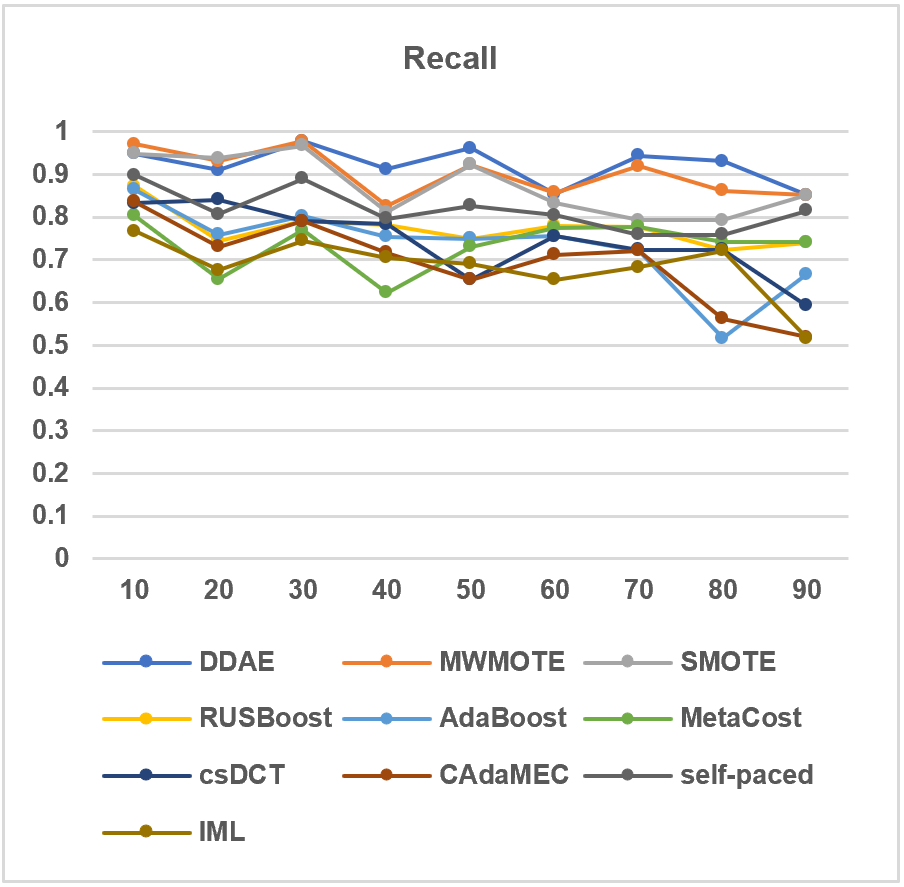
\includegraphics[width=\textwidth]{images/fig13}
        \caption{Recall: Impact of Imbalance Ratio}
        \label{fig13}
    \end{minipage}
    \quad
    \begin{minipage}{0.45\textwidth}
        \vspace{9.5pt}
        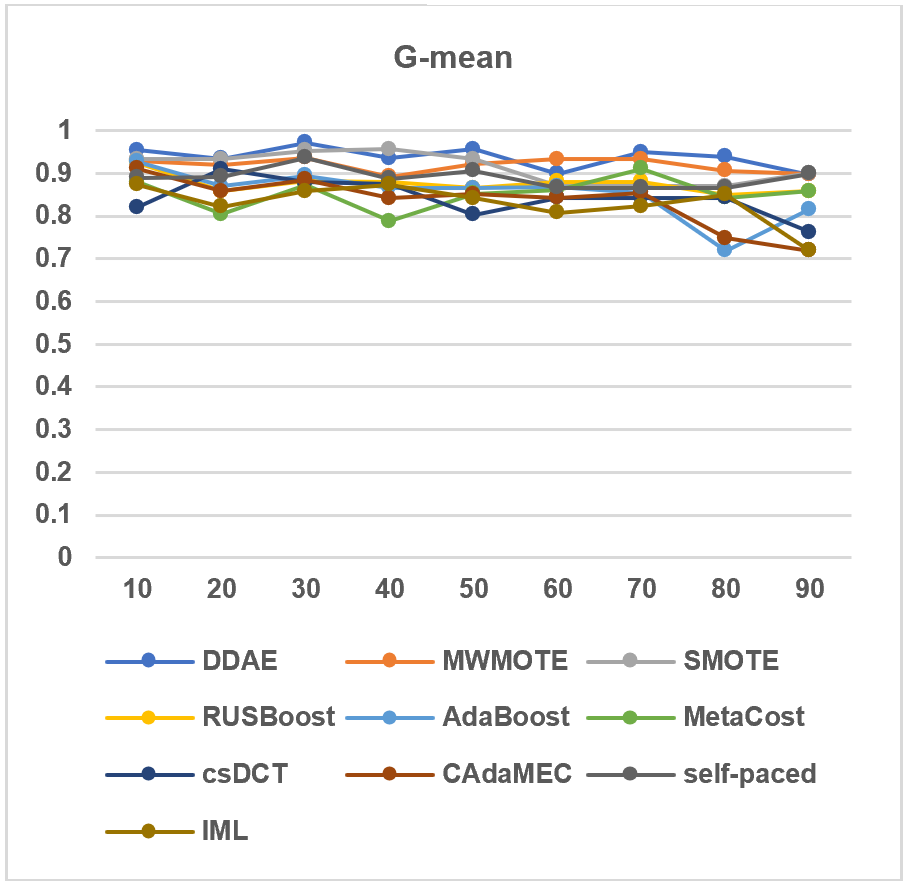
\includegraphics[width=\textwidth]{images/fig15}
        \caption{G-mean: Impact of Imbalance Ratio}
        \label{fig15}
    \end{minipage}
\end{figure}

Figure \ref{fig13} illustrates the trend of recall of all algorithms as the IR increases. Clearly, this metric stays stable on DDAE most of the time, and DDAE keeps the recall between 0.9 and 0.95. MWMOTE, SMOTE, cost-sensitive Decision Tree, CAdaMEC, self-paced Ensemble Classifier and IML show a downward trend. Among these, the recall of MWMOTE, SMOTE and self-paced Ensemble Classifier decreased slightly as the class distribution became more imbalanced, with the highest and lowest values for MWMOTE, SMOTE, AdaBoost and self-paced Ensemble Classifier being 0.978(IR=30) and 0.852 (IR=90), 0.967 (IR=30) and 0.793 (IR=80), 0.865 (IR=10) and 0.517 (IR=80), 0.898 (IR=10) and 0.795 (IR=80), respectively. The figures for recall of the other four ``decreasing'' algorithms drop significantly, from 0.841 (IR=20) to 0.593 (IR=90) for csDCT, from 0.836 (IR=10) to 0.519 (IR=90) for CAdaMEC, and from 0.767 (IR=10) to 0.517 (IR=90) for IML. In addition, no obvious correlation between recall and the changes in IR can be seen through the curves of RUSBoost and MetaCost. All of them show a slight fluctuation in this process.

% The impact of IR on the precision of these models can be viewed in Figure \ref{fig14}. More than half of all models show a decrease as the IR climbs up, including DDAE, MWMOTE, SMOTE, csDCT and self-paced Ensemble Classifier. The difference between maximum and minimum for these models is 0.548, 0.374, 0.416, 0.577 and 0.442, respectively. In contrast, the figure for RUSBoost goes up after IR is greater than 30. Even though the curves of CAdaMEC and MetaCost are fluctuant, they still decrease slightly. Moreover, the precision of IML and AdaBoost maintain stability during the whole experiment, with the precision generally above 0.9 for both of the models.

Notably, the G-mean of almost all the models remain nearly stable with the exception of MetaCost. All of the models still retain a high value for G-mean even when the IR is 70 or 80. It can be observed from Figure \ref{fig15} that some of models performs better (or similarly) when the IR is 70 compared to the IR is 10, including DDAE, MWMOTE, SMOTE, RUSBoost, AdaBoost, MetaCost, self-paced Ensemble Classifier, IML and csDCT. 




% RUSBoost and AdaBoost show a decrease when the IR is greater than 80 and 70, respectively. 


% \begin{figure}[h]
%     \centering 
%     % \begin{minipage}{0.31\textwidth}
%     %     \centering
%     %     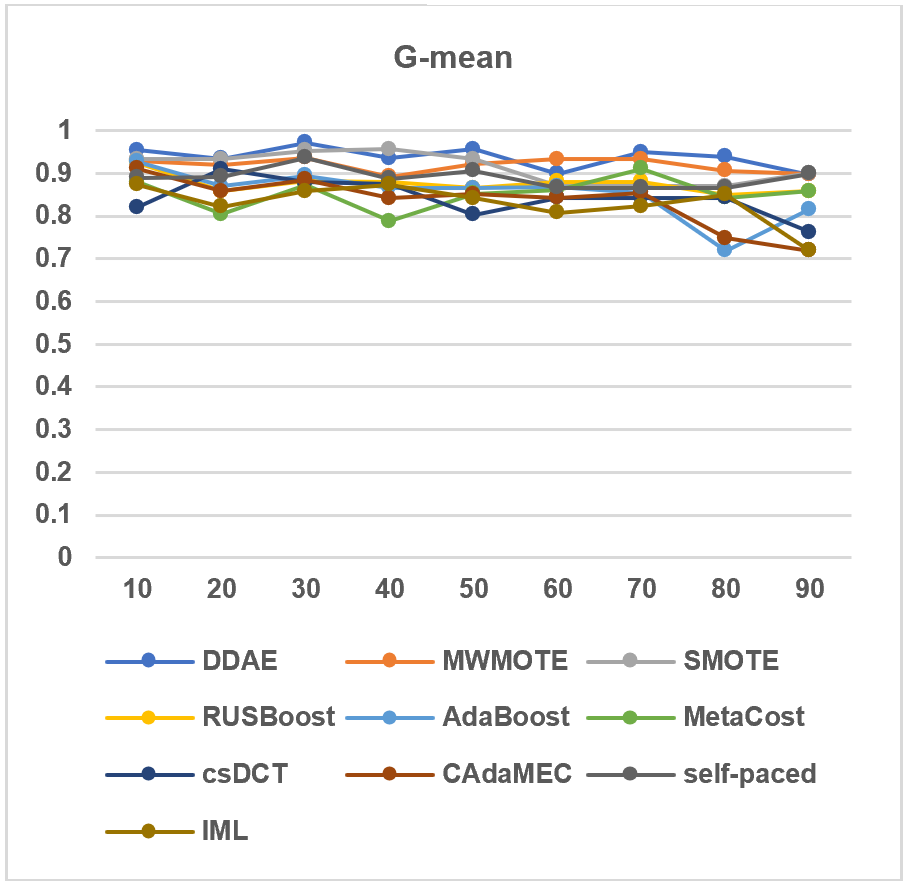
\includegraphics[width=\textwidth]{images/fig15}
%     %     \caption{G-mean: Impact of Imbalance Ratio}
%     %     \label{fig15}
%     % \end{minipage}
%     % \hspace{5pt}
%     \begin{minipage}{0.45\textwidth}
%         \centering
%         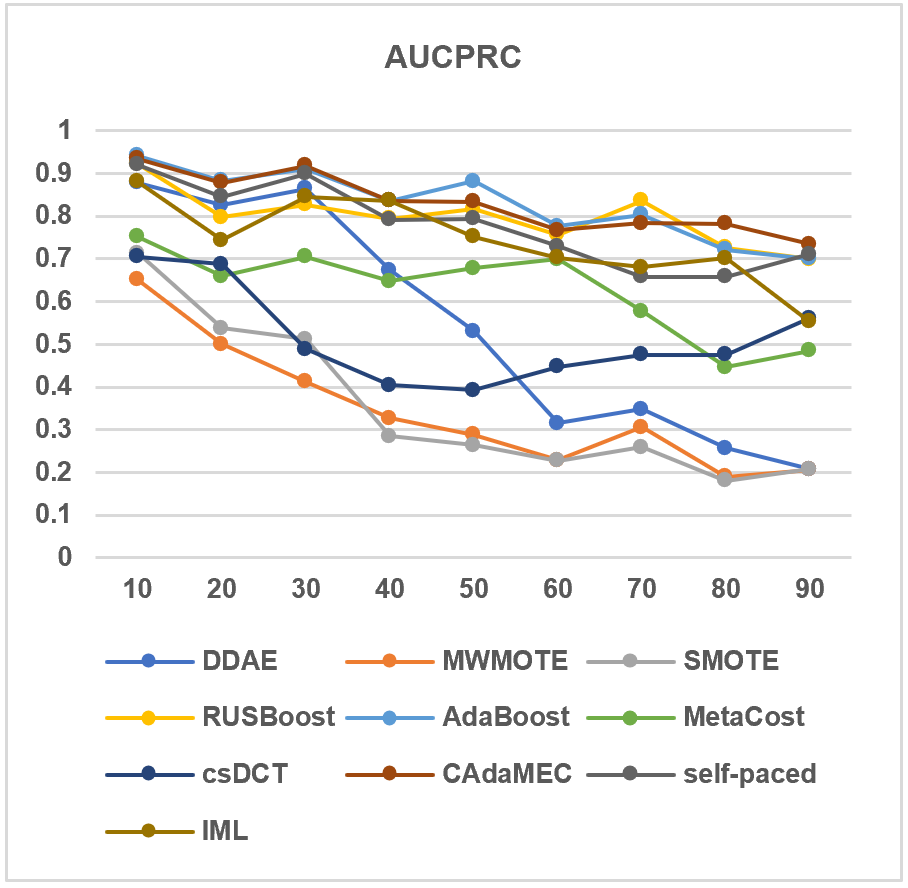
\includegraphics[width=\textwidth]{images/fig16}
%         \caption{AUCPRC: Impact of Imbalance Ratio}
%         \label{fig16}
%     \end{minipage}
%     \quad
%     \begin{minipage}{0.45\textwidth}
%         \vspace{9.5pt}
%         % \centering
%         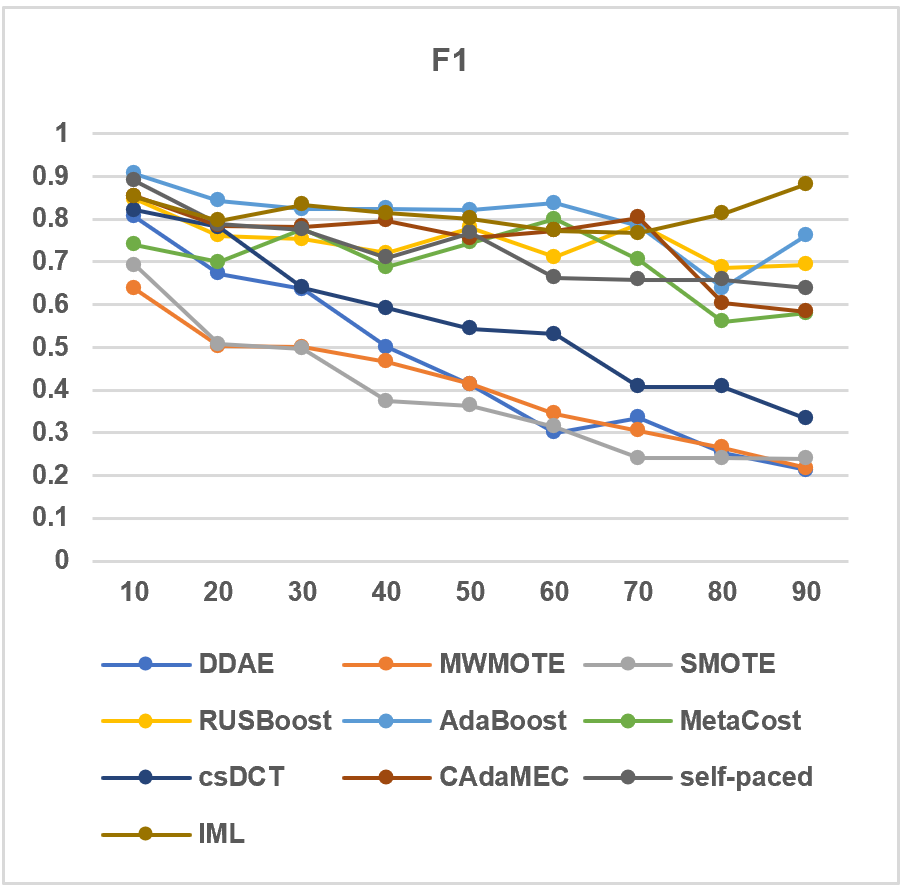
\includegraphics[width=\textwidth]{images/fig17}
%         \caption{F1: Impact of Imbalance Ratio}
%         \label{fig17}
%     \end{minipage}
% \end{figure}
\begin{figure}[h]
    \centering 
    \begin{minipage}[t]{0.45\textwidth}
        \vspace{0pt}
        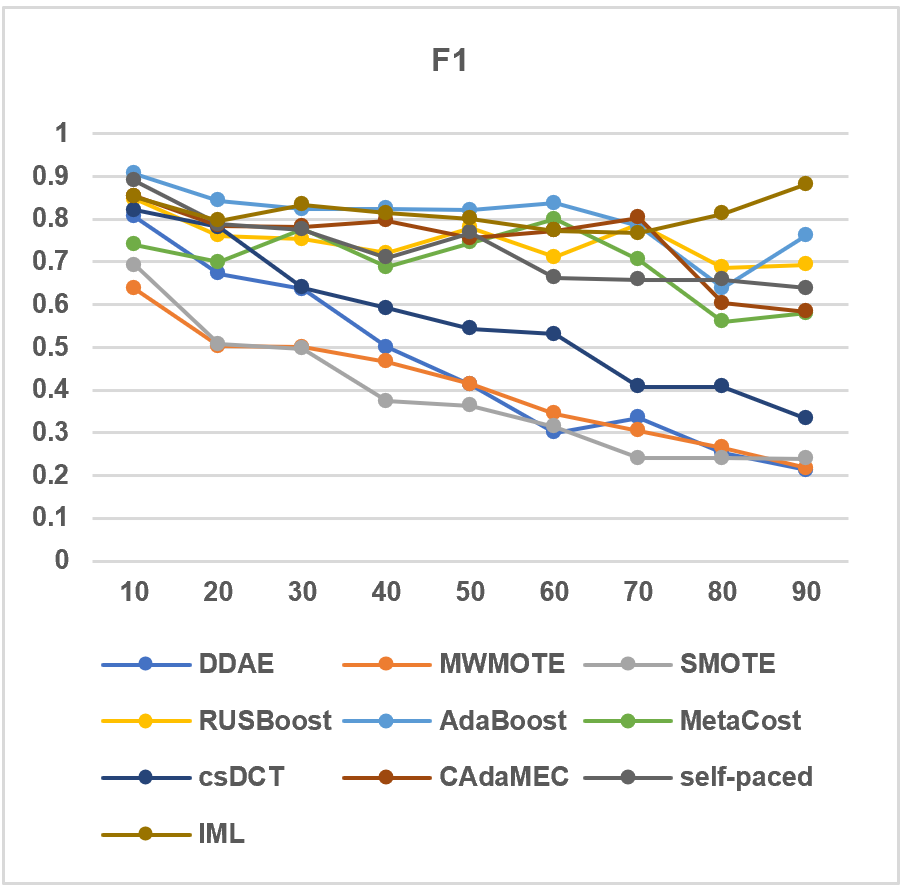
\includegraphics[width=\textwidth]{images/fig17}
        \caption{F1: Impact of Imbalance Ratio}
        \label{fig17}
    \end{minipage}
    \quad
    \begin{minipage}[t]{0.45\textwidth}
        \vspace{0pt}
        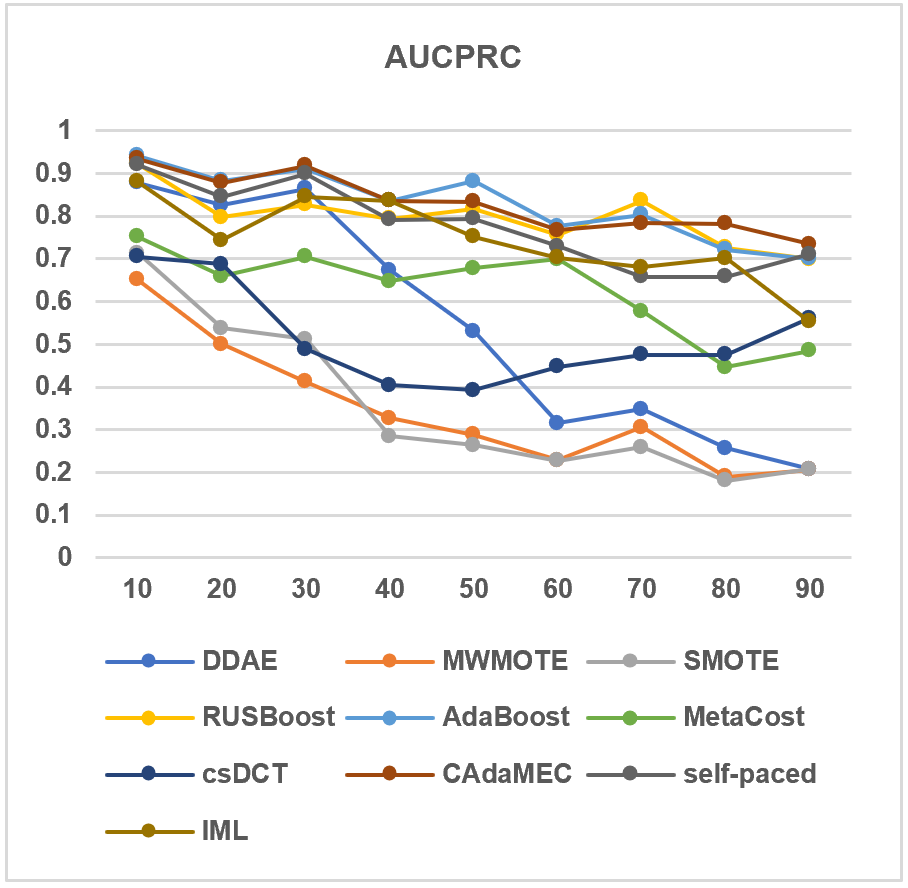
\includegraphics[width=\textwidth]{images/fig16}
        \caption{AUCPRC: Impact of Imbalance Ratio}
        \label{fig16}
    \end{minipage}
\end{figure}

F1 is the evaluation metric which takes both recall and precision into account, which means that if the trend of recall for one specific model maintain stability with only a slight decrease/increase, the changes in F1 will be similar to those in precision. According to the above description of the changes in recall, the trends for F1 of SMOTE, MWMOTE, DDAE, csDCT can be compared with those for their precision, which can be observed from Figure \ref{fig17}. The value of F1 for MetaCost and AdaBoost decrease slightly during the process. In contrast, as the performance of other models shows degradation to some degree, the figures for IML, RUSBoost and self-paced Ensemble Classifier stay almost stable, but the former increases slightly after IR is greater than 70 and the latter drops to a small degree. AUCPRC is another evaluation metric which considers recall and precision at the same time. According to Figure \ref{fig16}, the AUCPRCs for DDAE, MWMOTE, SMOTE, CAdaMEC and IML decrease as the IR increases. The figure for MetaCost fluctuates significantly but is still showing a decrease. The AUCPRCs for AdaBoost, RUSBoost and self-paced Ensemble Classifier are all on a slightly downward trend. Moreover, csDCT preforms differently on AUCPRC from other models, the figure for these two models climbing when the IR varies from 50 to 90. 

\subsection{Impact of the Size of Datasets}



% \begin{figure}[h]
%     \centering 
%     \begin{minipage}{0.31\textwidth}
%         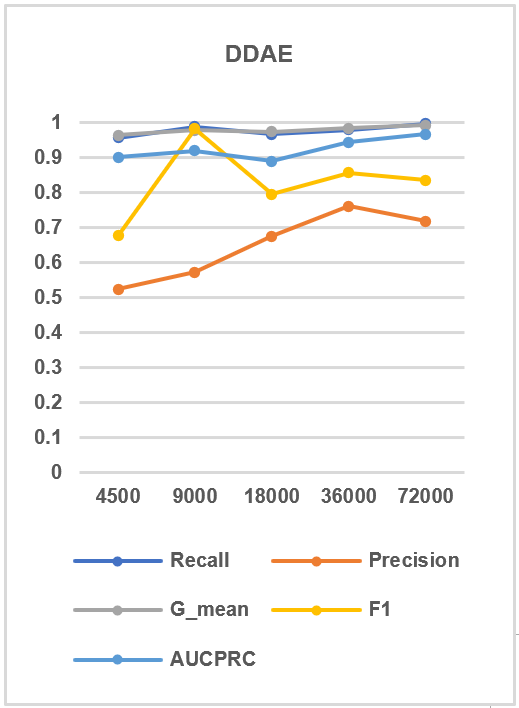
\includegraphics[width=\textwidth]{images/fig18}
%         \caption{DDAE: Impact of the Size of Dataset}
%         \label{fig18}
%     \end{minipage}
%     \begin{minipage}{0.31\textwidth}
%         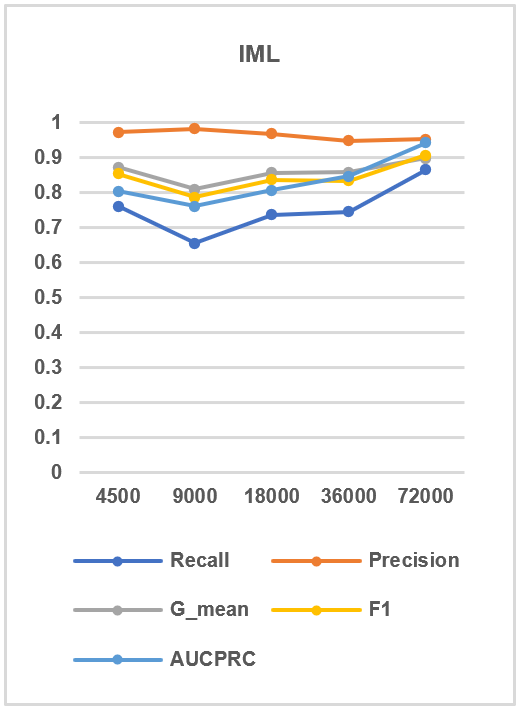
\includegraphics[width=\textwidth]{images/fig19}
%         \caption{IML: Impact of the Size of Dataset}
%         \label{fig19}
%     \end{minipage}
%     \begin{minipage}{0.31\textwidth}
%         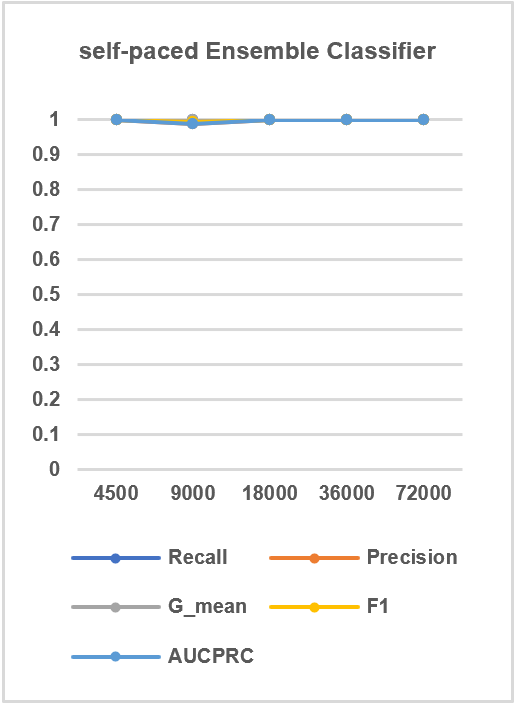
\includegraphics[width=\textwidth]{images/fig20}
%         \caption{self-paced: Impact of the Size of Dataset}
%         \label{fig20}
%     \end{minipage}

%     \begin{minipage}{0.31\textwidth}
%         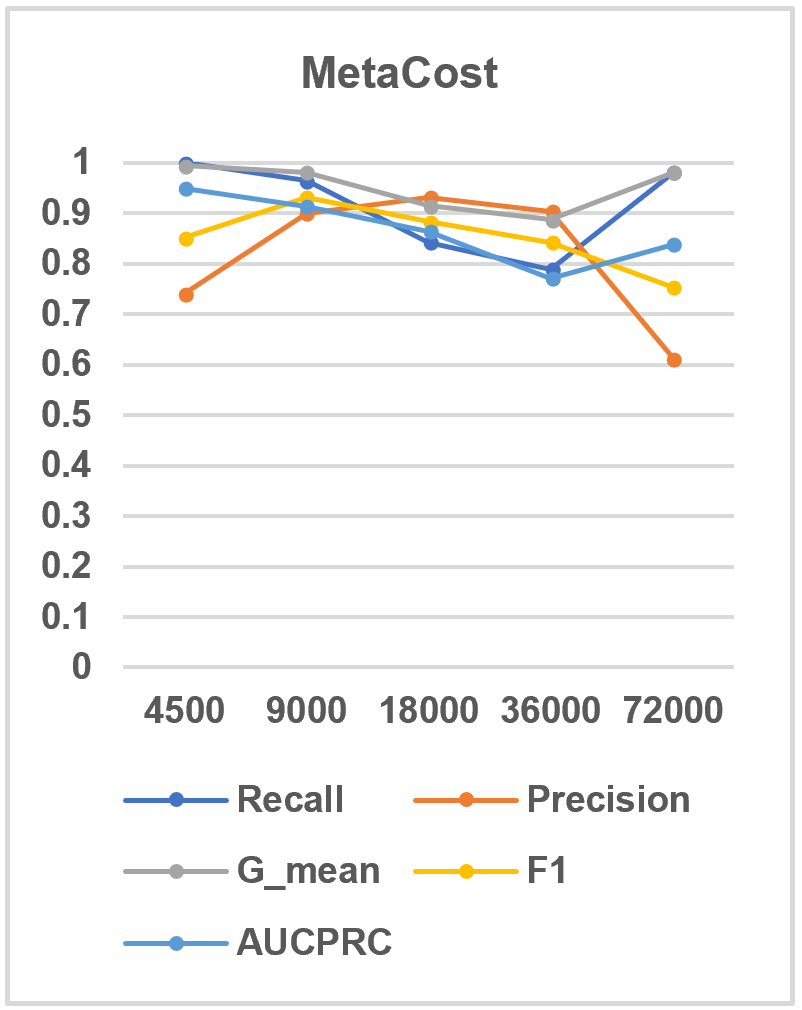
\includegraphics[width=\textwidth]{images/fig21}
%         \caption{MetaCost: Impact of the Size of Dataset}
%         \label{fig21}
%     \end{minipage}
%     \begin{minipage}{0.31\textwidth}
%         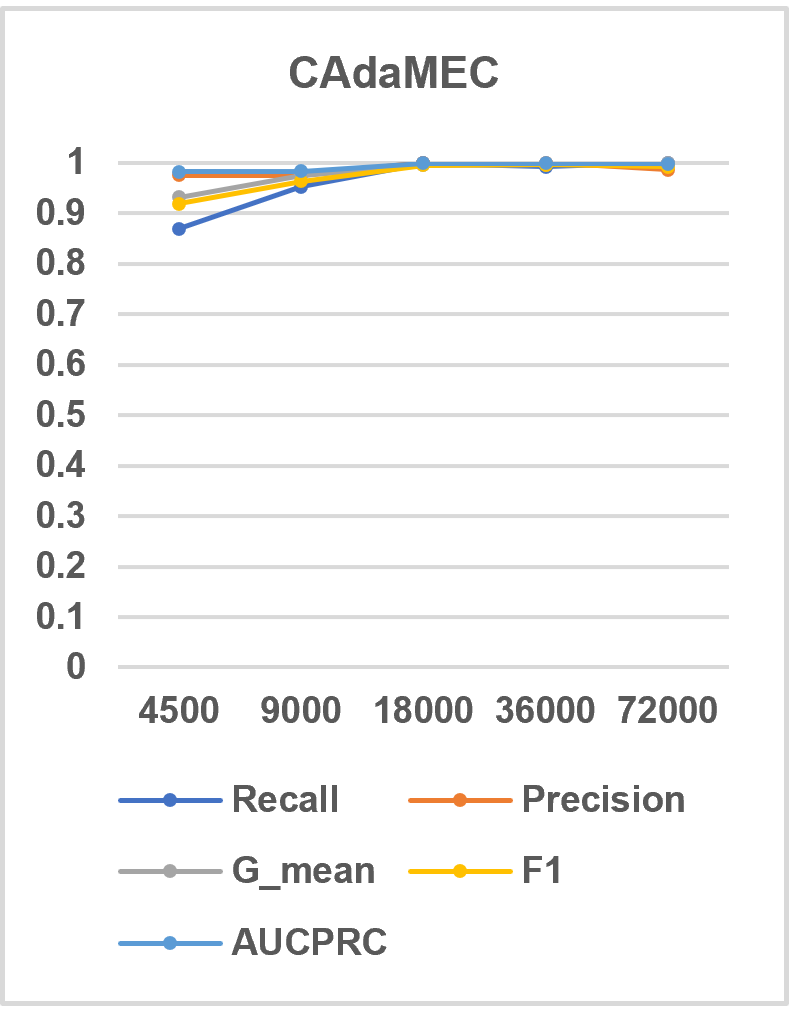
\includegraphics[width=\textwidth]{images/fig22}
%         \caption{CAdaMEC: Impact of the Size of Dataset}
%         \label{fig22}
%     \end{minipage}
%     \begin{minipage}{0.31\textwidth}
%         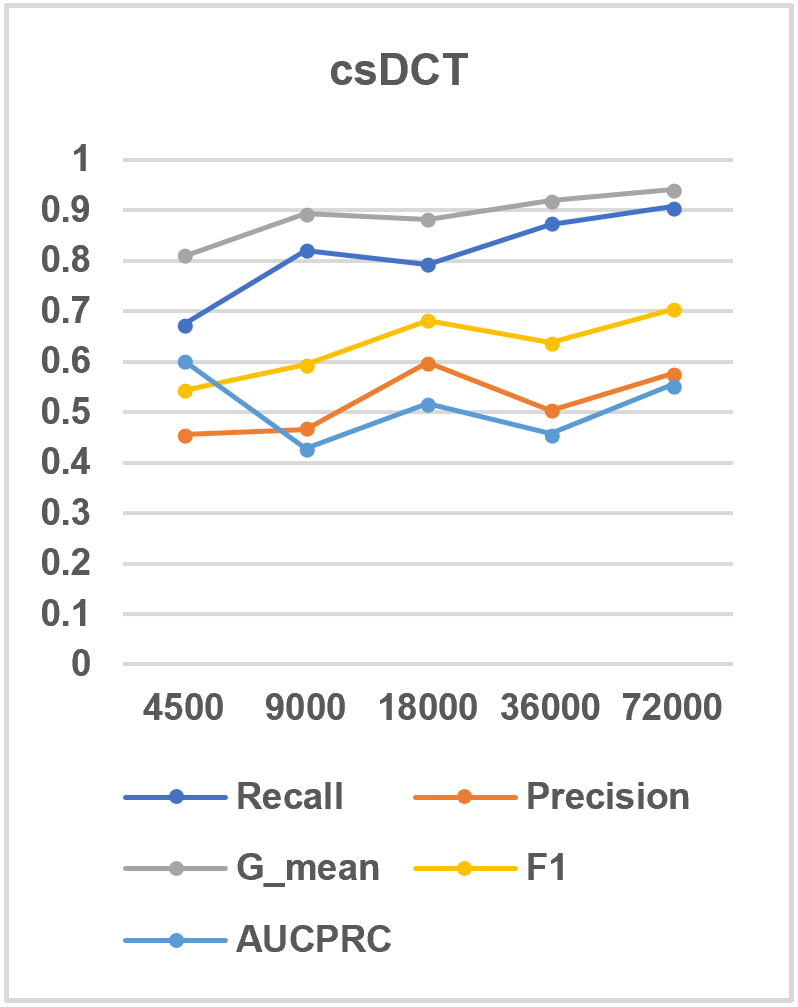
\includegraphics[width=\textwidth]{images/fig23}
%         \caption{csDCT: Impact of the Size of Dataset}
%         \label{fig23}
%     \end{minipage}

%     \begin{minipage}{0.31\textwidth}
%         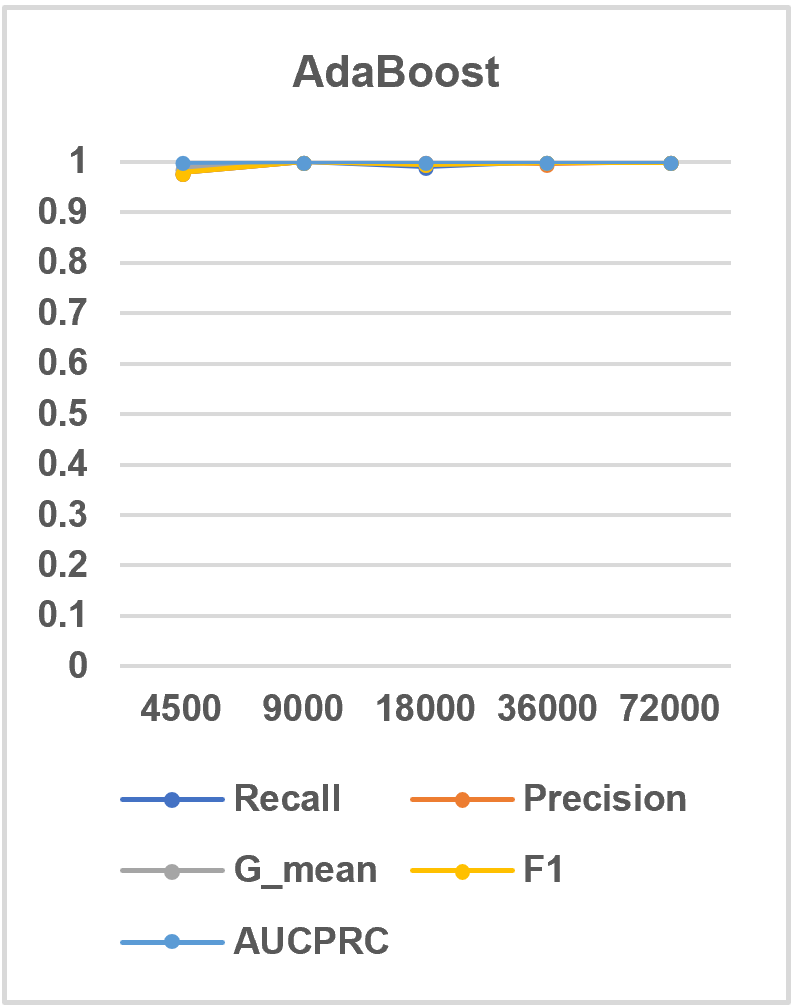
\includegraphics[width=\textwidth]{images/fig24}
%         \caption{AdaBoost: Impact of the Size of Dataset}
%         \label{fig24}
%     \end{minipage}
%     \begin{minipage}{0.31\textwidth}
%         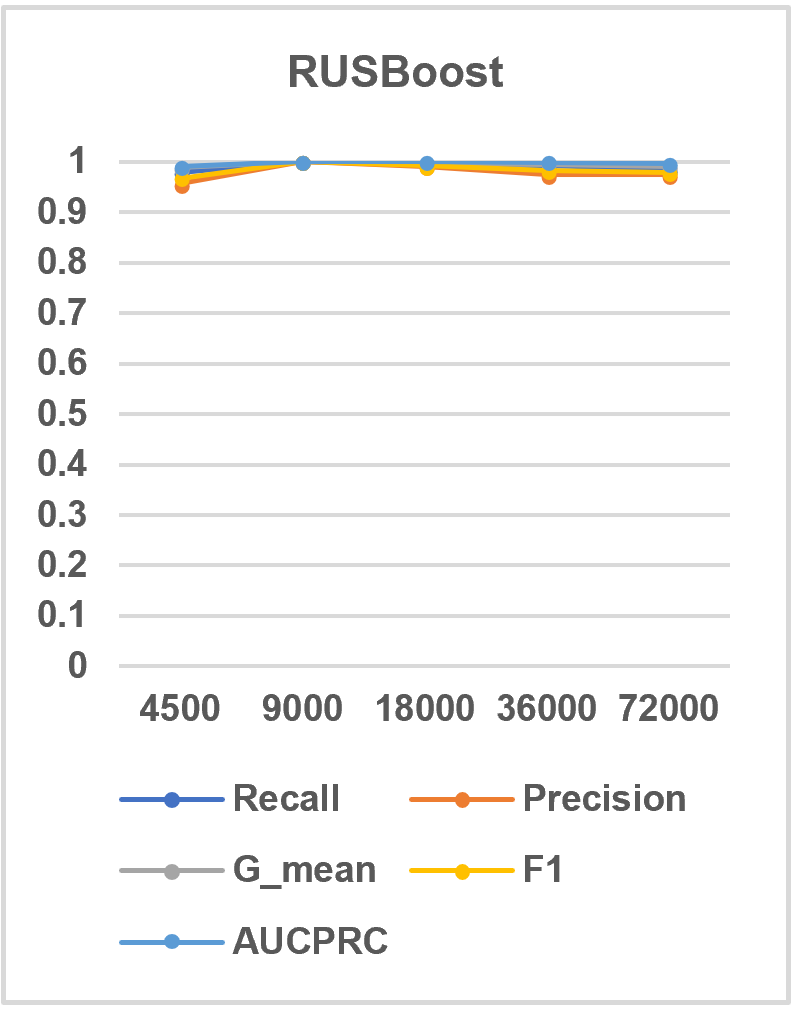
\includegraphics[width=\textwidth]{images/fig25}
%         \caption{RUSBoost: Impact of the Size of Dataset}
%         \label{fig25}
%     \end{minipage}
%     \begin{minipage}{0.31\textwidth}
%         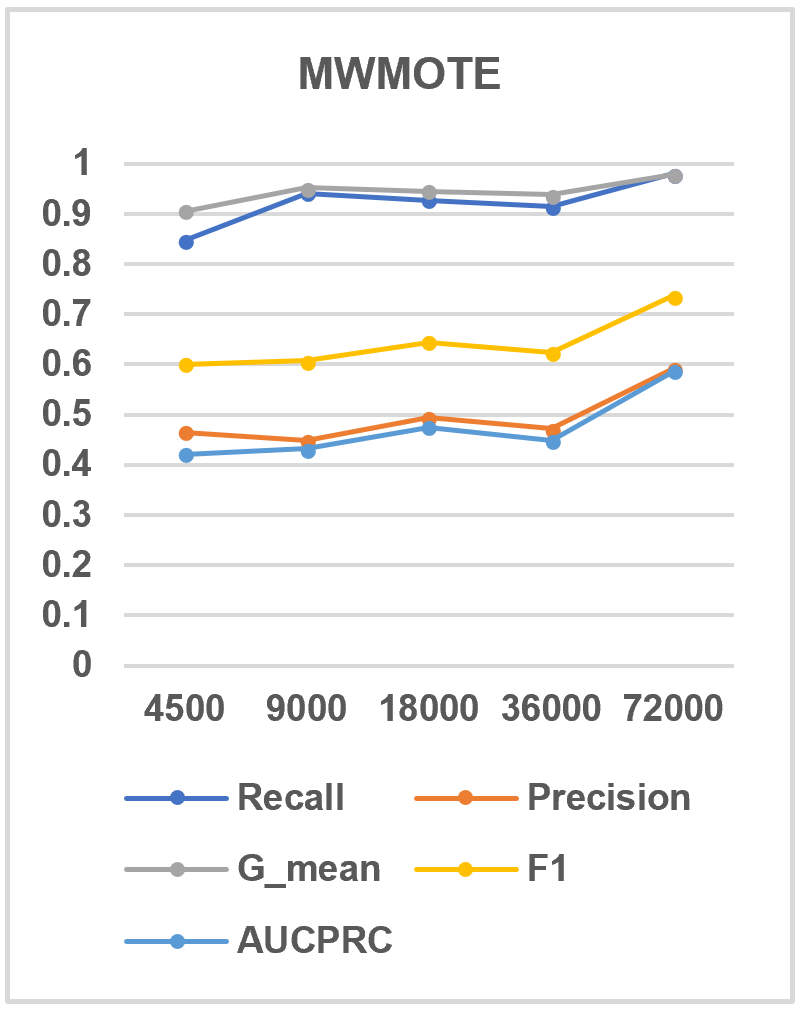
\includegraphics[width=\textwidth]{images/fig26}
%         \caption{MWMOTE: Impact of the Size of Dataset}
%         \label{fig26}
%     \end{minipage}

%     \begin{minipage}{0.31\textwidth}
%         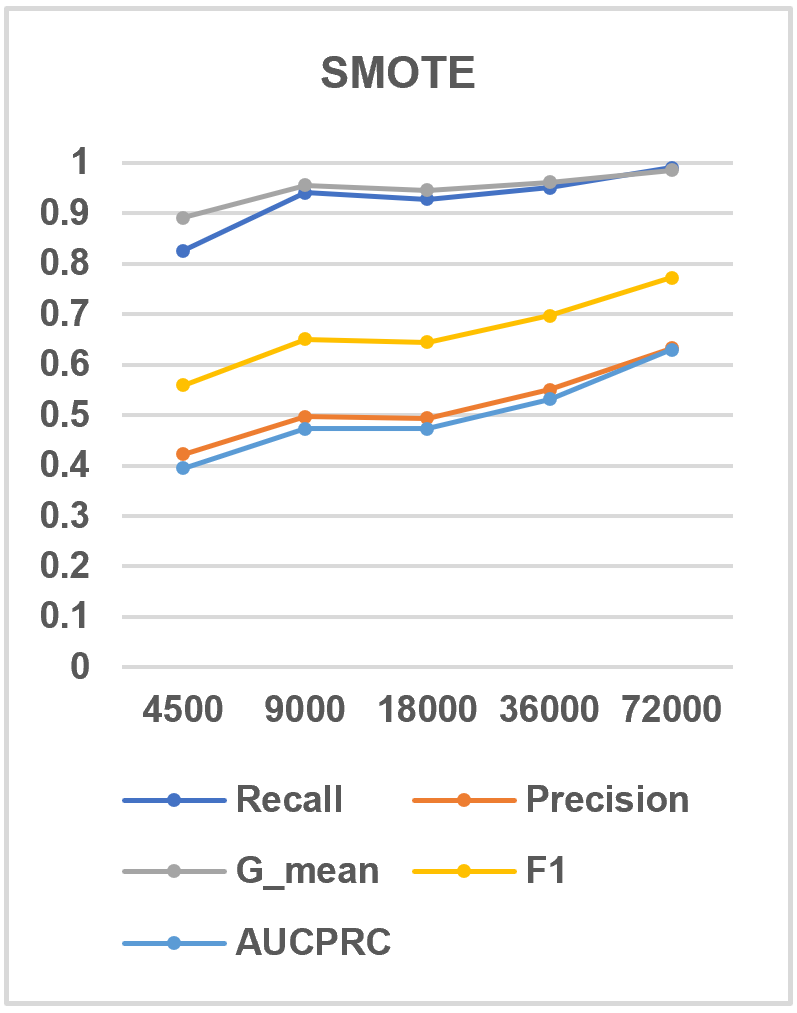
\includegraphics[width=\textwidth]{images/fig27}
%         \caption{IML: Impact of the Size of Dataset}
%         \label{fig27}
%     \end{minipage}
% \end{figure}

\begin{figure}[H]
    \centering 
    \begin{minipage}{0.31\textwidth}
        \centering
        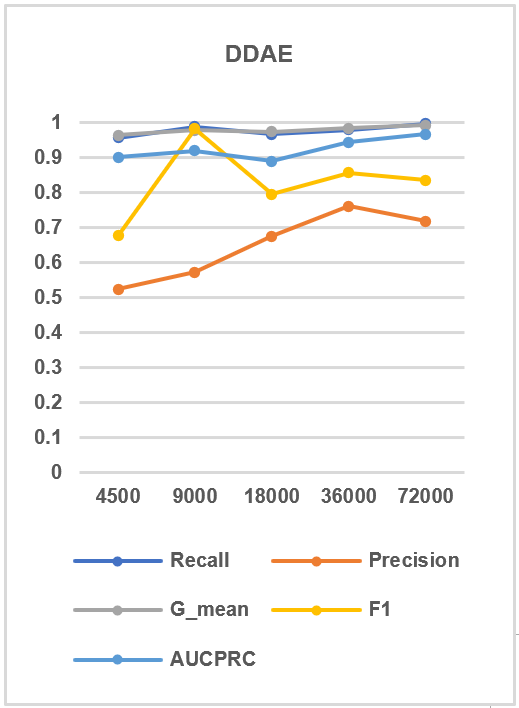
\includegraphics[width=0.8\textwidth]{images/fig18}
        \caption{DDAE: Impact of the Size of Dataset}
        \label{fig18}
    \end{minipage}
    \hspace{5pt}
    \begin{minipage}{0.31\textwidth}
        \centering
        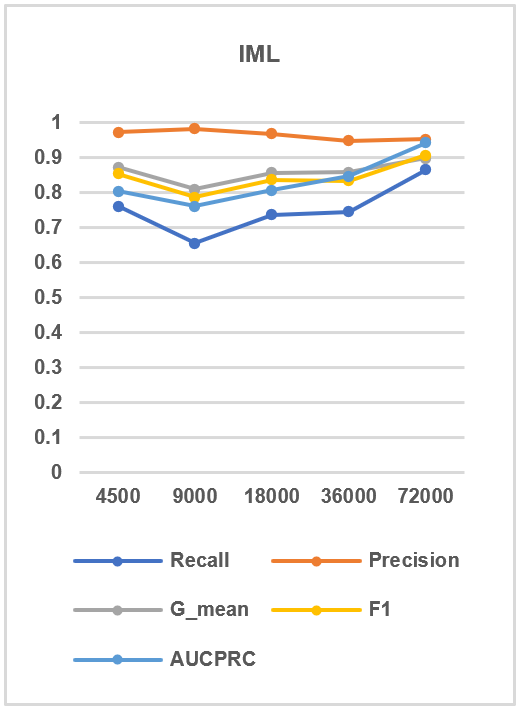
\includegraphics[width=0.8\textwidth]{images/fig19}
        \caption{IML: Impact of the Size of Dataset}
        \label{fig19}
    \end{minipage}
    \hspace{5pt}
    \begin{minipage}{0.31\textwidth}
        \centering
        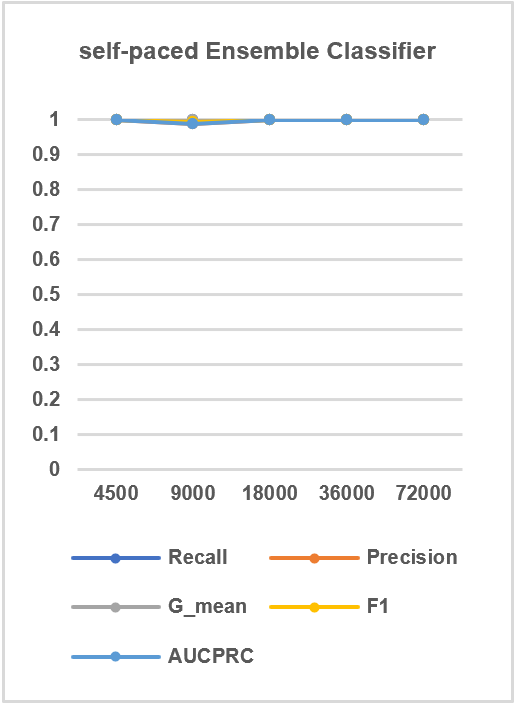
\includegraphics[width=0.8\textwidth]{images/fig20}
        \caption{self-paced: Impact of the Size of Dataset}
        \label{fig20}
    \end{minipage}
\end{figure}
\vspace{-10pt}

\begin{figure}[h]
    \centering 
    \begin{minipage}{0.31\textwidth}
        \centering
        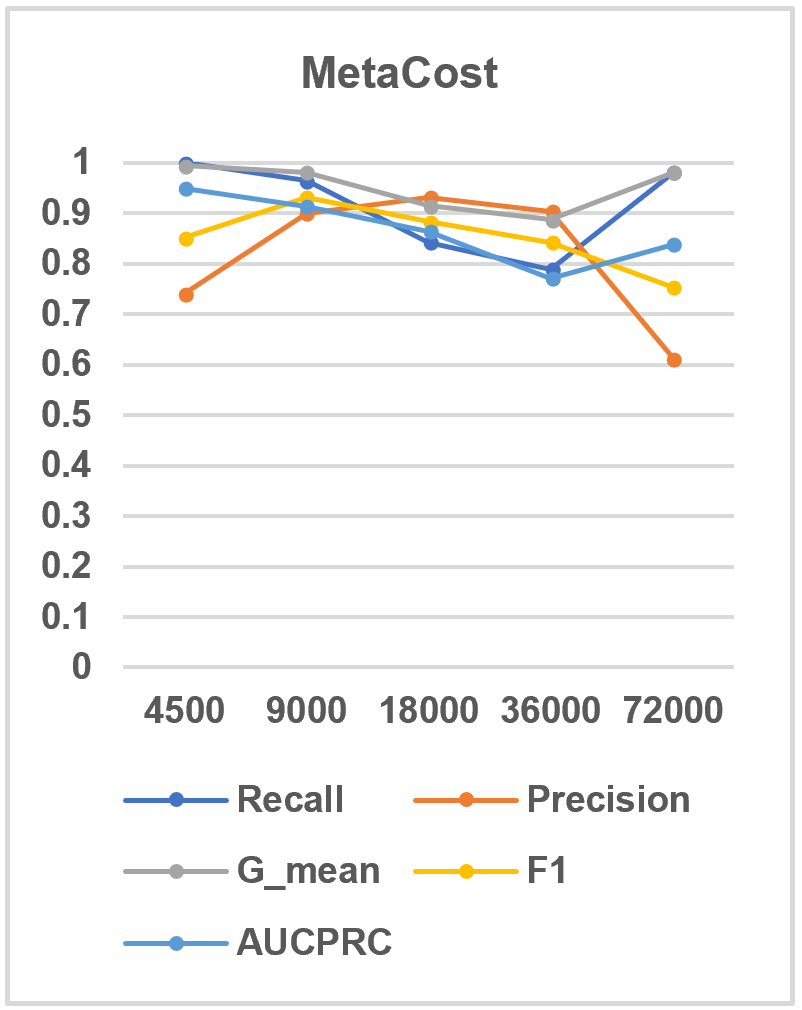
\includegraphics[width=0.8\textwidth]{images/fig21}
        \caption{MetaCost: Impact of the Size of Dataset}
        \label{fig21}
    \end{minipage}
    \hspace{5pt}
    \begin{minipage}{0.31\textwidth}
        \centering
        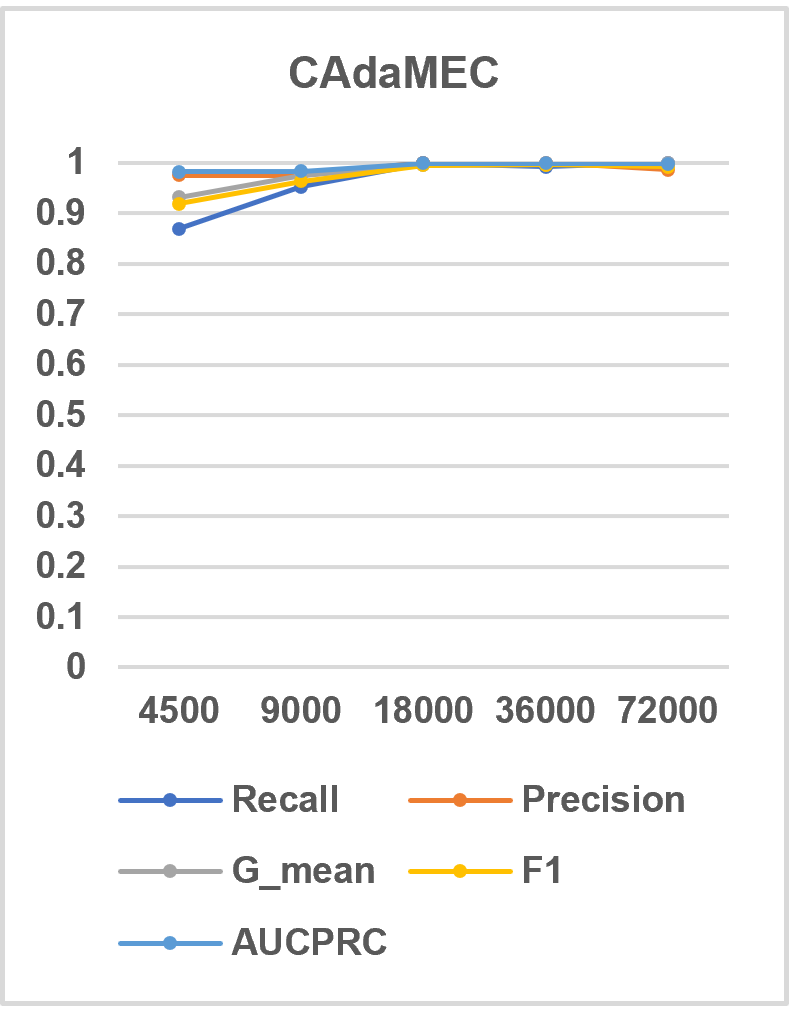
\includegraphics[width=0.8\textwidth]{images/fig22}
        \caption{CAdaMEC: Impact of the Size of Dataset}
        \label{fig22}
    \end{minipage}
    \hspace{5pt}
    \begin{minipage}{0.31\textwidth}
        \centering
        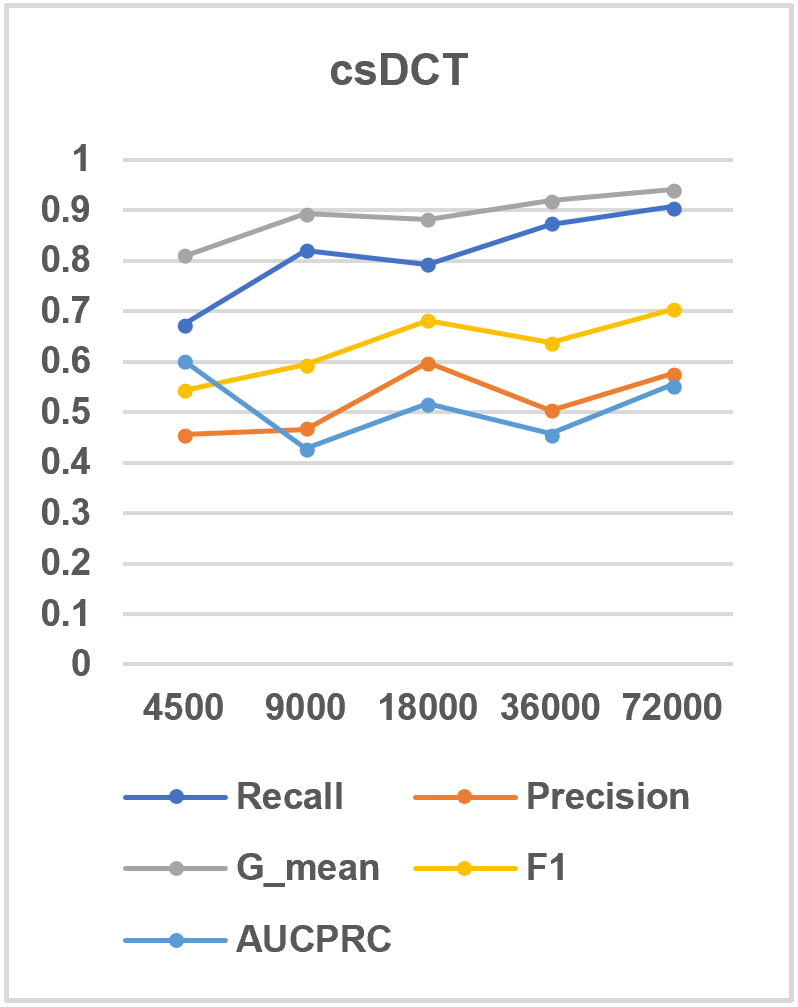
\includegraphics[width=0.8\textwidth]{images/fig23}
        \caption{csDCT: Impact of the Size of Dataset}
        \label{fig23}
    \end{minipage}
\end{figure}
\vspace{-10pt}

\begin{figure}[H]
    \centering 
    \begin{minipage}{0.31\textwidth}
        \centering
        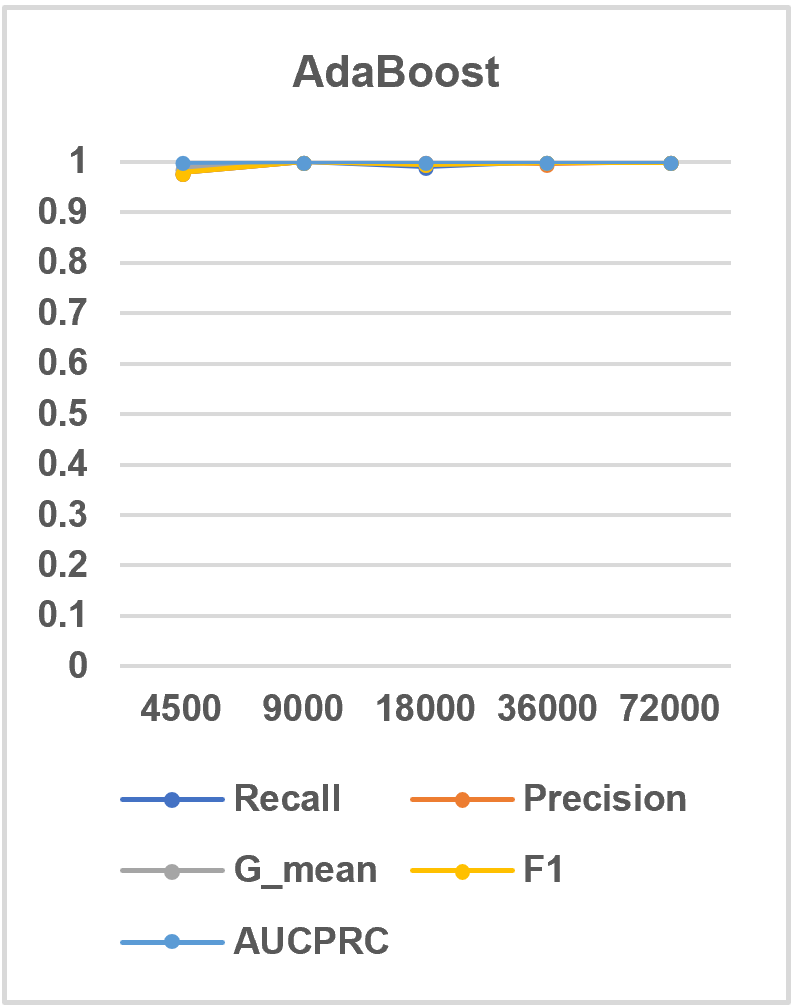
\includegraphics[width=0.8\textwidth]{images/fig24}
        \caption{AdaBoost: Impact of the Size of Dataset}
        \label{fig24}
    \end{minipage}
    \hspace{5pt}
    \begin{minipage}{0.31\textwidth}
        \centering
        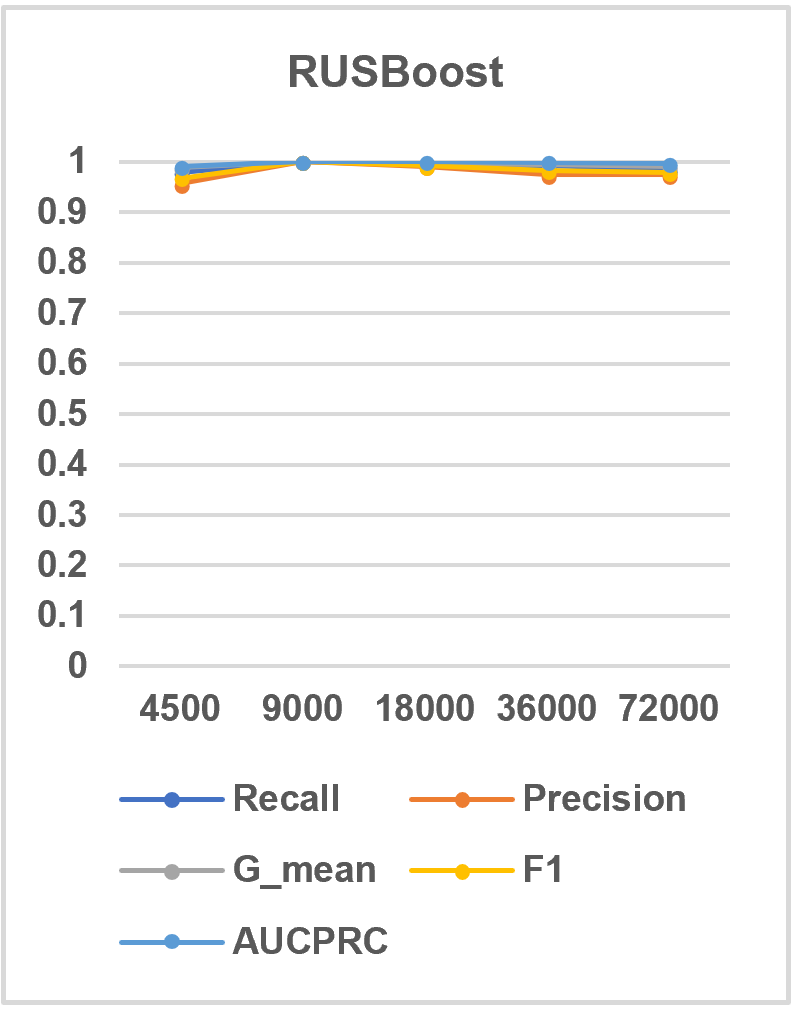
\includegraphics[width=0.8\textwidth]{images/fig25}
        \caption{RUSBoost: Impact of the Size of Dataset}
        \label{fig25}
    \end{minipage}
    \hspace{5pt}
    \begin{minipage}{0.31\textwidth}
        \centering
        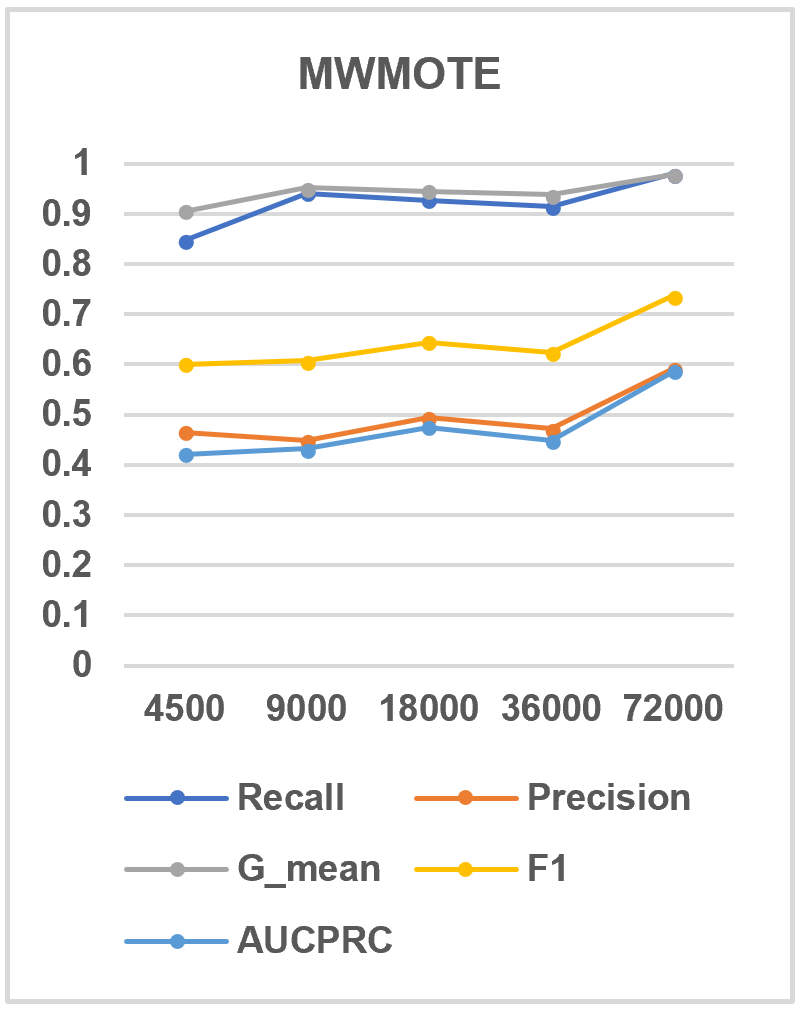
\includegraphics[width=0.8\textwidth]{images/fig26}
        \caption{MWMOTE: Impact of the Size of Dataset}
        \label{fig26}
    \end{minipage}
\end{figure}

\begin{figure}[H]
    \centering 
    \begin{minipage}{0.31\textwidth}
        \centering
        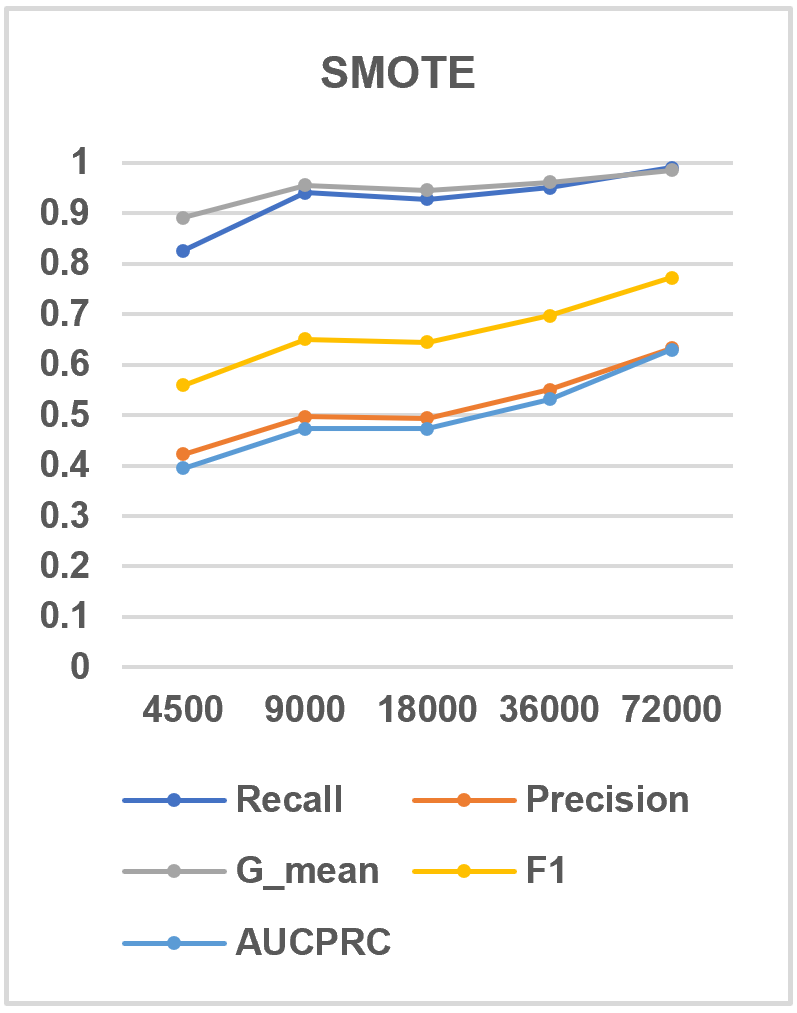
\includegraphics[width=0.8\textwidth]{images/fig27}
        \caption{SMOTE: Impact of the Size of Dataset}
        \label{fig27}
    \end{minipage}
\end{figure}

Next, in order to analyze whether the size of the dataset will affect the classification accuracy of the model, five sub-datasets with the same IR but a different number of instances (which are \#Instances=4500, 9000, 18000, 36000 and 72000) are taken from the Protein Homology dataset. The results can be observed in Figures \ref{fig18}-\ref{fig27}.

It can be seen from the figures that in the process of increasing the sample size of the algorithms DDAE, MWMOTE, SMOTE, IML and cost-sensitive Decision Tree (csDCT), the values of the five evaluation metrics have shown an upward trend, especially the precision and F1, which increases more than 0.2 and 0.1 respectively. This phenomenon shows that the classification results are more accurate on these models when the sample size is extensive compared to when the sample size is small.

The RUSBoost, AdaBoost, self-paced Ensemble Classifier and CAdaMEC algorithms are not significantly affected by the size of the dataset. The performance of the algorithms on all five experiments are quite excellent, and the value of the evaluation metrics are mostly between 0.9-1.0. Although the CAdaMEC is slightly inadequate when the total sample size is 4500, the recall value is also greater than 0.8, and as the total number of instances exceeds 10,000, this model can predict the labels of all majority and minority class correctly among all the algorithms. 

It can be noted that, only MetaCost does not show an apparent trend.

\section{Results on Effectiveness of DDAE}
\subsection{Results on Effectiveness of Components}
The DDAE model includes a total of four components, namely: Data Block Construction (DBC), Data Space Improvement (DSI), Adaptive Weight Adjustment (AWA) and Ensemble Learning (EL). In order to analyze the effectiveness of each component in the entire model, DDAE is modified by deleting the components except for EL in the model. After that, three variants are created: DDAE-DBC, DDAE-AWA and DDAE-DSI. It should be noted that since DDAE itself is an ensemble model, EL is indispensable at all times, which is why the DDAE-El is not listed in these variants. It can be observed from Figure \ref{fig27} and Figure \ref{fig28} that on two datasets (PH1 and Euthyroid Sick) when the model removes the DBC module, the recall and G-mean drops significantly, which is the poorest performance among all variants and the original model. At the same time, it can be seen that the precision varies distinctly across the variants. But the recall of DDAE without AWA or DSI does not drop as much. The performance of the original model without DSI also can be affected, which can be observed from the Figure \ref{fig27} and Figure\ref{fig28} for all evaluation metrics. Without the improvement to data space, the accuracy of prediction may decrease. All in all, the integrated algorithm of DDAE absorbs the advantages of each component so that the minority classes can be correctly classified.
\begin{figure}[h]
    \centering 
    \begin{minipage}{0.45\textwidth}
        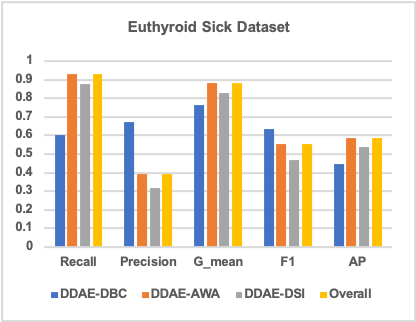
\includegraphics[width=\textwidth]{images/fig28}
        \caption{Effectiveness of DDAE on Euthyroid Sick Dataset}
        \label{fig28}
    \end{minipage}
    \quad
    \begin{minipage}{0.45\textwidth}
        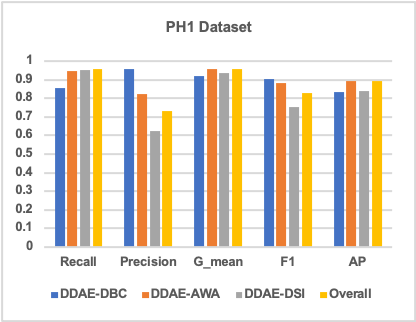
\includegraphics[width=\textwidth]{images/fig29}
        \caption{Effectiveness of DDAE on PH1 Dataset}
        \label{fig29}
    \end{minipage}
\end{figure}

\subsection{Impact of Parameters}
In this section, the impact of parameters(including the number of blocks in DBC, the relative weight between pull and push in DSI, the unstable ratio and the cost ratio in AWA) on the DDAE model is analyzed through a set of experiments. These experiments are conducted on the Cm1 and Mw1 dataset.

\begin{figure}[h]
    \centering 
    \begin{minipage}{0.45\textwidth}
        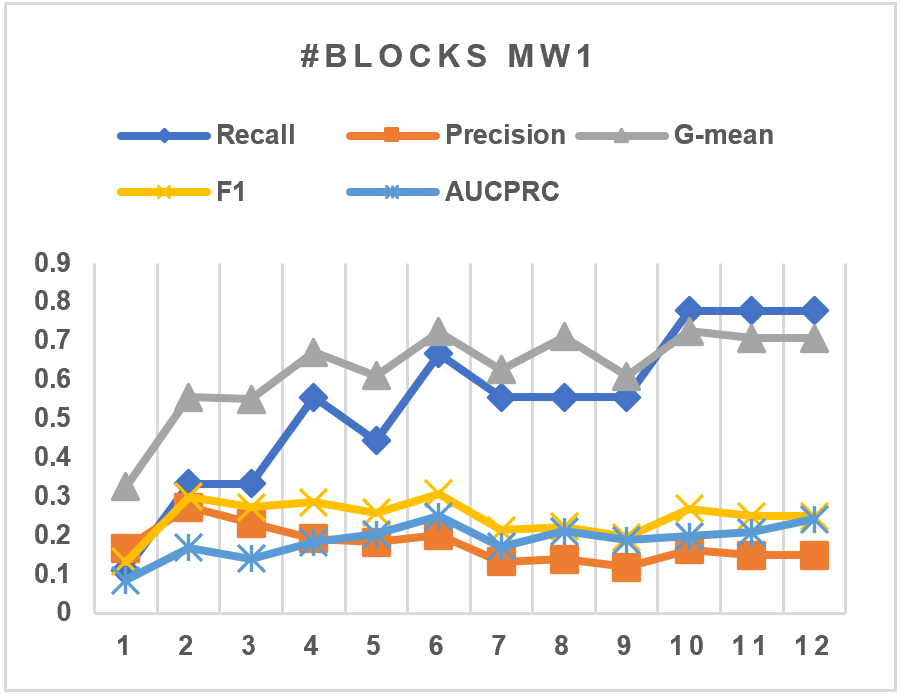
\includegraphics[width=\textwidth]{images/fig30}
        \caption{Impact of the Number of Data Blocks on Mw1}
        \label{fig30}
    \end{minipage}
    \quad
    \begin{minipage}{0.45\textwidth}
        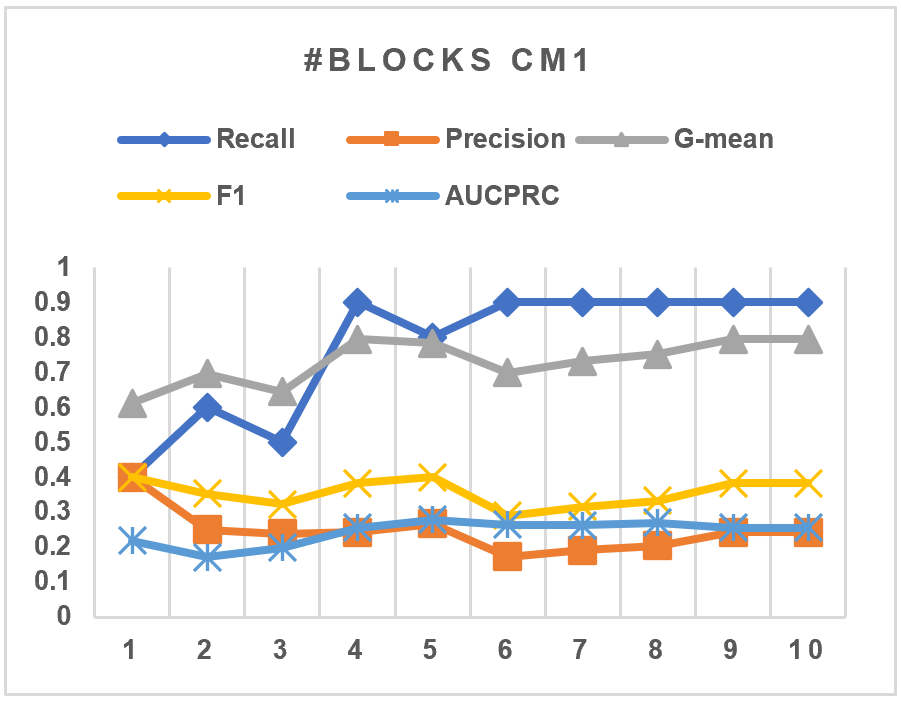
\includegraphics[width=\textwidth]{images/fig31}
        \caption{Impact of the Number of Data Blocks on Cm1}
        \label{fig31}
    \end{minipage}
\end{figure}

\subsubsection{Impact of the Number of Split Data Blocks in DBC}
The data blocks in DBC are utilized to adjust the imbalanced sample distribution so that each data block can reach a balanced level. As illustrated in Figure \ref{fig30} and Figure \ref{fig31}, a similar trend is shared among these evaluation metrics as the number of data blocks grows. It can be observed that the model works better when the number of data blocks is close to the imbalance ratio(IR(Cm1) = 10, IR(Mw1) = 12).


\subsubsection{Impact of the Relative Weight between the Pull and Push Terms in DSI}
In this section, the impact of relative weight $\omega$ between the pull and push terms in DSI is analyzed by varying $\omega$ from 0.1 to 1 on the Cm1 and Mw1 dataset. Notably, the Figure \ref{fig32} and Figure \ref{fig33} illustrate how the model achieves the best performance on Cm1 when $\omega=0.1$ and on Mw1 when $\omega=0.3$. Due to the specific data distribution on each dataset, the best choice of $\omega$ can differ.


\begin{figure}[h]
    \centering 
    \begin{minipage}{0.45\textwidth}
        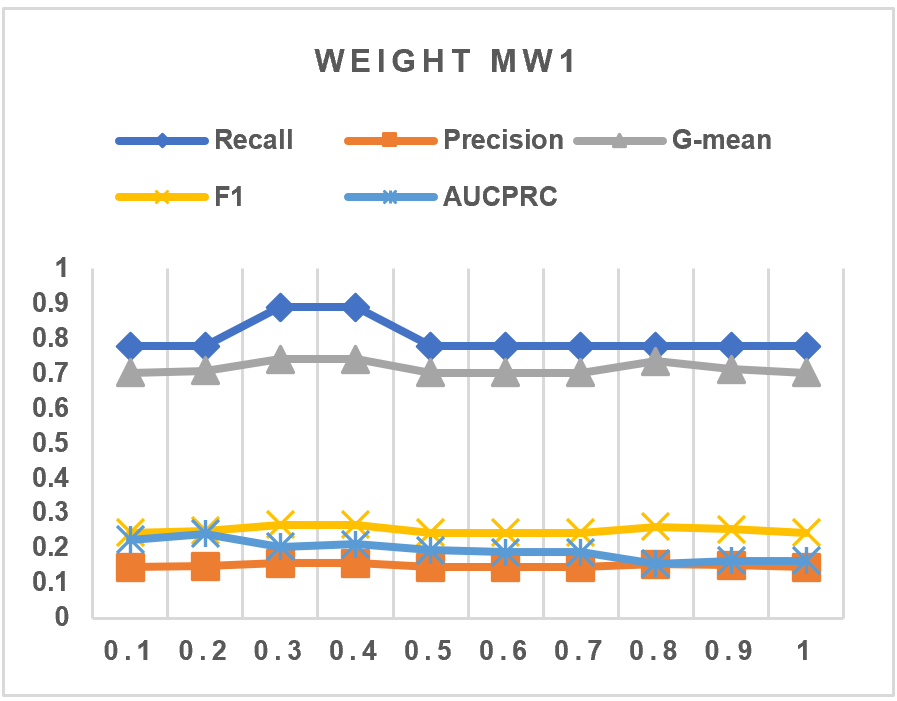
\includegraphics[width=\textwidth]{images/fig32}
        \caption{Impact of the relative Weight between the Pull and Push Terms on Mw1}
        \label{fig32}
    \end{minipage}
    \quad
    \begin{minipage}{0.45\textwidth}
        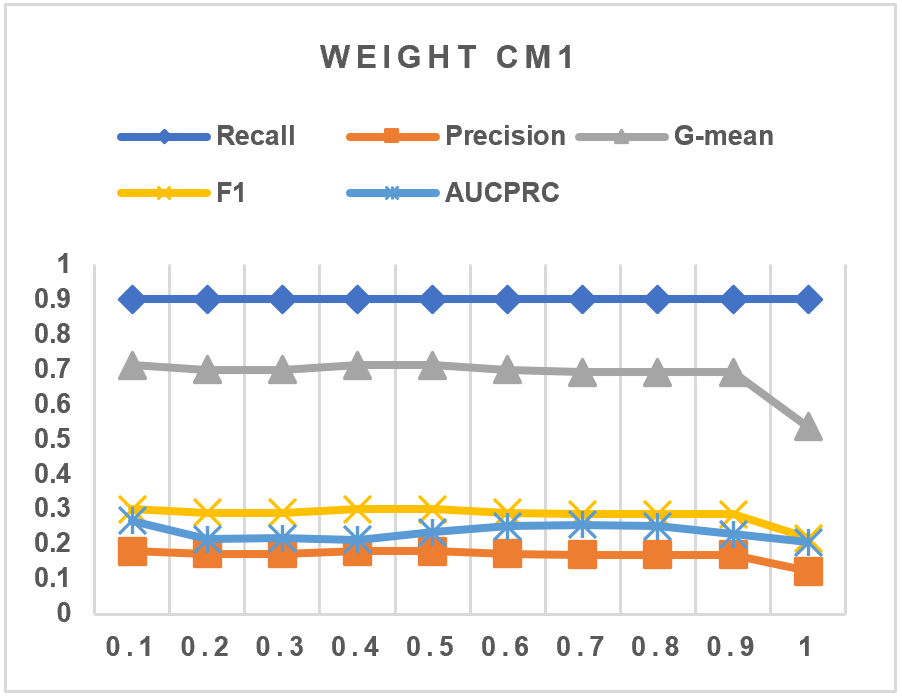
\includegraphics[width=\textwidth]{images/fig33}
        \caption{Impact of the relative Weight between the Pull and Push Terms on Cm1}
        \label{fig33}
    \end{minipage}
\end{figure}

\subsubsection{Impact of the Unstable Ratio in AWA}
% The unstable ratio $\tau$ from AWA is a threshold term that is utilized to help determine whether the AWA generated weight pair should be considered in the decision or not. In order to locate the optimal value for $\tau$, it is varied from 0.1 to 1.0 on the two given datasets. It can be observed from Figure \ref{fig35} Impact of Unstable Ratio on CM1 and Figure \ref{fig34} Impact of Unstable Ratio on MW1 obviously that, from $\tau=0.3$, the trend of these four evaluation metrics become stable and unchanged. The model achieves the best performance on Cm1 and Mw1 dataset when $\tau=0.2$ and $\tau=0.3$, respectively.
\begin{figure}[H]
    \centering 
    \begin{minipage}{0.45\textwidth}
        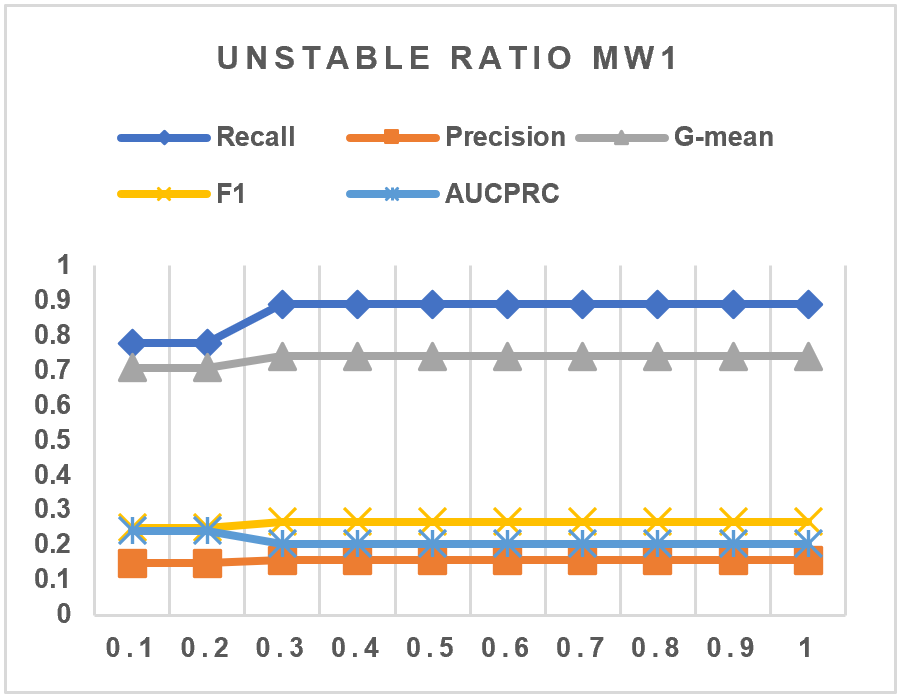
\includegraphics[width=\textwidth]{images/fig34}
        \caption{Impact of Unstable Ratio on Mw1}
        \label{fig34}
    \end{minipage}
    \quad
    \begin{minipage}{0.45\textwidth}
        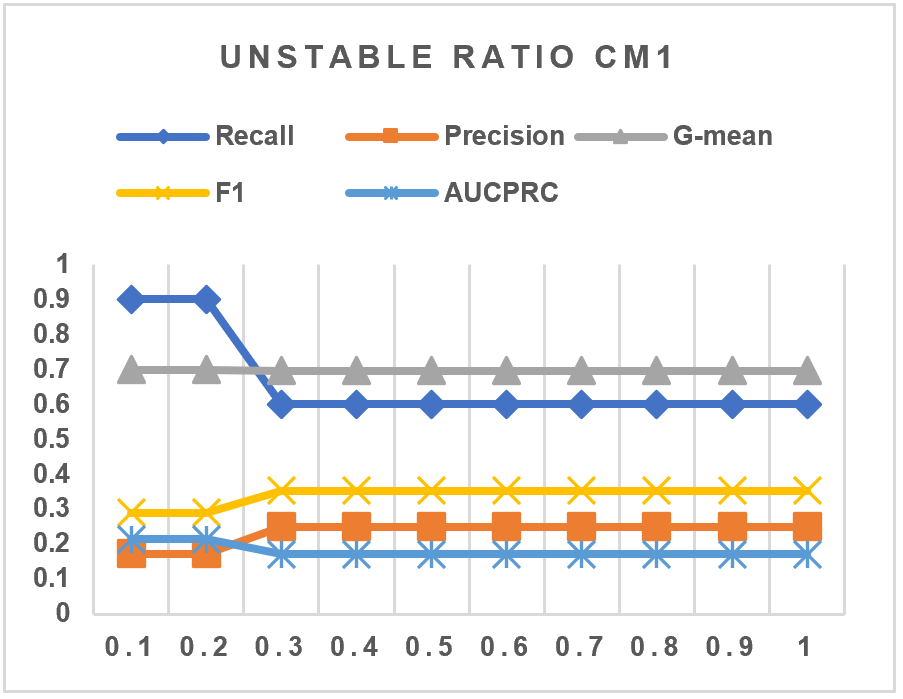
\includegraphics[width=\textwidth]{images/fig35}
        \caption{Impact of Unstable Ratio on Cm1}
        \label{fig35}
    \end{minipage}
\end{figure}
The unstable ratio $\tau$ from AWA is a threshold term that is utilized to help determine whether the AWA generated weight pair should be considered in the decision or not. In order to locate the optimal value for $\tau$, it is varied from 0.1 to 1.0 on the two given datasets. It can be clearly observed from Figure \ref{fig34} and Figure \ref{fig35} that, from $\tau=0.3$, the trend of these four evaluation metrics becomes stable and unchanged. The model achieves the best performance on the Cm1 and Mw1 datasets when $\tau=0.2$ and $\tau=0.3$, respectively.

\subsubsection{Impact of the Cost Ratio in AWA}
\begin{figure}[H]
    \centering 
    \begin{minipage}{0.45\textwidth}
        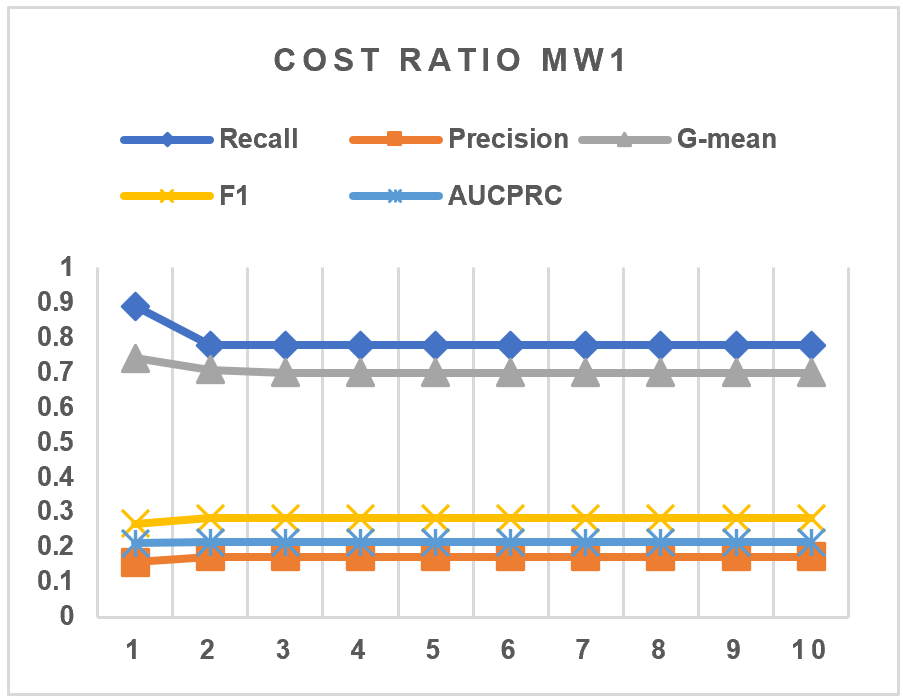
\includegraphics[width=\textwidth]{images/fig36}
        \caption{Impact of Cost Ratio on Mw1}
        \label{fig36}
    \end{minipage}
    \quad
    \begin{minipage}{0.45\textwidth}
        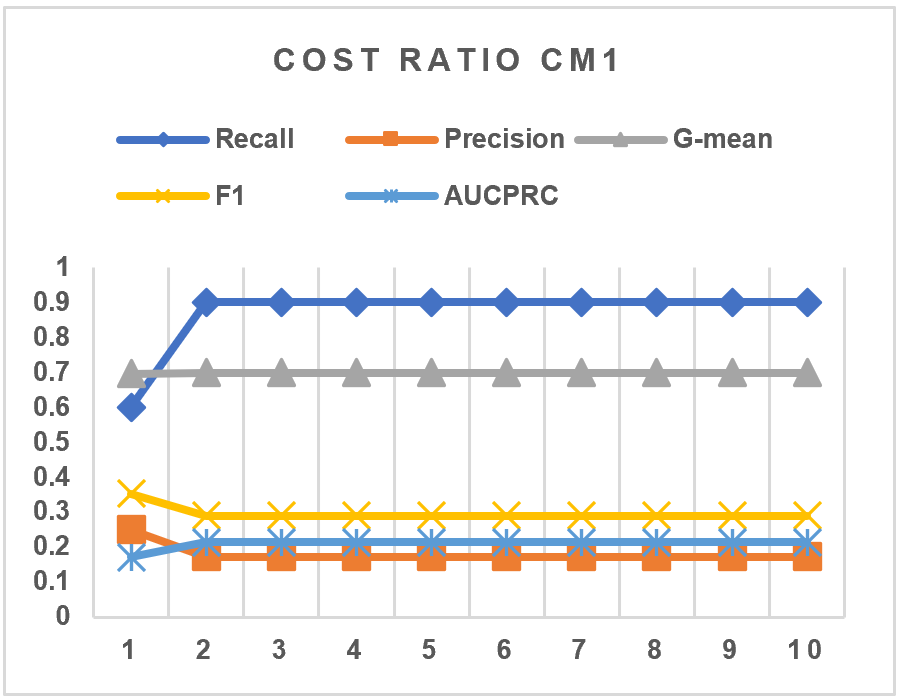
\includegraphics[width=\textwidth]{images/fig37}
        \caption{Impact of Cost Ratio on Cm1}
        \label{fig37}
    \end{minipage}
\end{figure}

As introduced in Chapter 2, the most significant step of the cost-sensitive learning method is choosing the cost for False Positive (FP) and False Negative (FN), and the cost ratio shows which class is more important in the classification process. But if there is no experts' suggestions or any other additional information related to these two classes, the decision of an appropriate cost ratio may become difficult. In this experiment, the tested range of cost ratio is from 1 to the imbalance ratio. For instance, cost ratio = 1 means the two classes are equally important. From Figure \ref{fig36} and Figure \ref{fig37}, it can be seen that, when the cost ratio is above 2, the performance of the model remains stable on both datasets. 